\documentclass[11pt,a4paper]{article}
% ============================================================
%  Shared preamble for the Medical Signal and Image Processing
%  Lab reports (English edition).  Compile with pdfLaTeX.
% ============================================================
\usepackage[T1]{fontenc}
\usepackage[utf8]{inputenc}
\usepackage{mathpazo}                     % Palatino text and math
\usepackage[scaled=0.92]{helvet}          % sans-serif for headings
\usepackage{courier}                      % monospace for code
\usepackage{amsmath,amssymb,bm}
\usepackage{microtype}
\usepackage[a4paper,left=2.4cm,right=2.4cm,top=2.9cm,bottom=2.5cm,headheight=22pt]{geometry}
\usepackage{xcolor}
\usepackage{graphicx}
\usepackage{float}
\usepackage{placeins}
\usepackage{booktabs,array,multirow,tabularx,longtable}
\usepackage{enumitem}
\usepackage{siunitx}
\usepackage{caption,subcaption}
\usepackage{fancyhdr}
\usepackage{titlesec}
\usepackage{listings}
\usepackage[most]{tcolorbox}
\usepackage{tikz}
\usepackage[colorlinks=true,linkcolor=primary,citecolor=primary,urlcolor=primary]{hyperref}

\linespread{1.06}
\setlength{\parindent}{0pt}
\setlength{\parskip}{0.55em}
\emergencystretch=3em

% ---------- colours ----------
\definecolor{primary}{HTML}{1B6B87}
\definecolor{accent}{HTML}{C2522B}
\definecolor{soft}{HTML}{EAF3F6}
\definecolor{ink}{HTML}{22313A}
\definecolor{muted}{HTML}{6B7A83}

% ---------- headings ----------
\titleformat{\section}
  {\sffamily\bfseries\LARGE\color{primary}}{\thesection}{0.7em}{}
  [{\vspace{-0.2em}\color{primary!35}\titlerule[0.8pt]}]
\titleformat{\subsection}
  {\sffamily\bfseries\large\color{ink}}{\thesubsection}{0.6em}{}
\titleformat{\subsubsection}
  {\sffamily\bfseries\normalsize\color{primary}}{\thesubsubsection}{0.5em}{}
\titlespacing*{\section}{0pt}{1.6em}{0.9em}
\titlespacing*{\subsection}{0pt}{1.3em}{0.5em}
\titlespacing*{\subsubsection}{0pt}{1.0em}{0.3em}

% ---------- header / footer ----------
\pagestyle{fancy}
\fancyhf{}
\renewcommand{\headrulewidth}{0.4pt}
\renewcommand{\headrule}{\hbox to\headwidth{\color{primary!45}\leaders\hrule height \headrulewidth\hfill}}
\fancyhead[L]{\sffamily\small\color{muted}Medical Signal and Image Processing Lab}
\fancyhead[R]{\sffamily\small\color{muted}\reportshorttitle}
\fancyfoot[C]{\sffamily\small\color{muted}\thepage}
\fancypagestyle{plain}{\fancyhf{}\fancyfoot[C]{\sffamily\small\color{muted}\thepage}\renewcommand{\headrulewidth}{0pt}}

% ---------- captions ----------
\captionsetup{font={small,sf},labelfont={bf,color=primary},labelsep=period,
  format=plain,justification=centering,skip=6pt}
\captionsetup[table]{position=above,skip=5pt}
\renewcommand{\arraystretch}{1.18}

% ---------- code listings ----------
\lstdefinestyle{code}{
  basicstyle=\ttfamily\footnotesize,
  keywordstyle=\color{primary}\bfseries,
  commentstyle=\color{muted}\itshape,
  stringstyle=\color{accent},
  backgroundcolor=\color{soft},
  frame=single, rulecolor=\color{primary!30},
  framerule=0.5pt, xleftmargin=0pt, framexleftmargin=4pt,
  aboveskip=0.8em, belowskip=0.6em, breaklines=true,
  showstringspaces=false, columns=fullflexible, keepspaces=true,
  upquote=true, tabsize=2}
\lstset{style=code}

% ---------- boxes ----------
\newtcolorbox{keyresult}[1][]{enhanced,breakable,
  colback=soft,colframe=primary,boxrule=0pt,
  borderline west={3pt}{0pt}{primary},
  arc=2pt,left=10pt,right=10pt,top=7pt,bottom=7pt,
  fonttitle=\sffamily\bfseries,coltitle=primary,
  attach boxed title to top left={yshift=-2mm,xshift=0mm},
  boxed title style={colback=white,boxrule=0pt,top=0pt,bottom=0pt,left=0pt},
  #1}
\newtcolorbox{notebox}[1][]{enhanced,breakable,
  colback=white,colframe=accent!70,boxrule=0pt,
  borderline west={3pt}{0pt}{accent},
  arc=2pt,left=10pt,right=10pt,top=6pt,bottom=6pt,#1}
\newtcolorbox{taskbox}[1][Task]{enhanced,breakable,
  colback=black!4,colframe=black!4,boxrule=0pt,
  borderline west={2.5pt}{0pt}{muted},
  arc=1pt,left=9pt,right=9pt,top=5pt,bottom=5pt,
  fontupper=\small,
  title={\sffamily\bfseries\scriptsize\textcolor{muted}{\MakeUppercase{#1}}},
  coltitle=muted,fonttitle=\sffamily\bfseries\scriptsize,
  attach title to upper={\par\smallskip}}
\newcommand{\pending}[1]{%
  \begin{tcolorbox}[enhanced,colback=white,colframe=white,boxrule=0pt,
    borderline={0.6pt}{0pt}{muted,dashed},arc=2pt,left=8pt,right=8pt,top=5pt,bottom=5pt]
    \sffamily\small\color{muted}Translation pending: #1
  \end{tcolorbox}}

% ---------- question / answer helpers ----------
\newcommand{\question}[2]{%
  \subsection*{\textcolor{accent}{Q#1}\texorpdfstring{\hspace{0.6em}}{ }#2}%
  \addcontentsline{toc}{subsection}{Q#1\texorpdfstring{\quad}{ }#2}}
\newcommand{\answer}{\textbf{\textsf{\textcolor{primary}{Answer.}}}\ }

% ---------- convenient units / symbols ----------
\newcommand{\mV}{\si{\milli\volt}}
\newcommand{\Hz}{\si{\hertz}}

% ---------- title page ----------
% needs: \reportnumber \reporttitle \reportsubtitle
%        \authorone \authortwo \instructor \semester  (authors.tex)
\newcommand{\makereporttitle}{%
  \begingroup
    \thispagestyle{empty}
    \centering
    \vspace*{1.2cm}
    
\includegraphics[width=3.2cm]{sharif-logo.png}\par\vspace{0.9cm}
    {\sffamily\bfseries\Large\color{ink}Sharif University of Technology\par}
    \vspace{0.3cm}
    {\sffamily\large\color{muted}Medical Signal and Image Processing Lab\par}
    \vspace{1.0cm}
    {\color{primary}\rule{0.55\textwidth}{1.2pt}\par}
    \vspace{1.0cm}
    {\sffamily\small\color{accent}\textls[150]{\MakeUppercase{\reportnumber}}\par}
    \vspace{0.5cm}
    {\sffamily\bfseries\fontsize{26}{31}\selectfont\color{primary}\reporttitle\par}
    \vspace{0.6cm}
    {\sffamily\large\color{ink}\reportsubtitle\par}
    \vspace{1.0cm}
    {\color{primary}\rule{0.55\textwidth}{1.2pt}\par}
    \vspace{1.6cm}
    {\sffamily\bfseries\color{muted}\small\textls[100]{PREPARED BY}\par}
    \vspace{0.4cm}
    {\sffamily\Large\color{ink}\authorone\par}
    \vspace{0.2cm}
    {\sffamily\Large\color{ink}\authortwo\par}
    \vspace{1.3cm}
    {\sffamily\color{muted}Instructor:\ \textbf{\color{ink}\instructor}\par}
    \vfill
    {\sffamily\color{muted}\semester\par}
    \vspace{0.8cm}
    \clearpage
  \endgroup}
% hyperlinked citation number (targets are defined in the reference list)
\newcommand{\refl}[1]{\hyperlink{ref:#1}{#1}}

% Author and course metadata (shared by all reports).
\newcommand{\authorone}{Mohammad Reza Mahdavi}
\newcommand{\authortwo}{Reza Kazemeini Moghaddam}
\newcommand{\instructor}{Marzieh Barakat}
\newcommand{\semester}{Fall Semester 2026}


\newcommand{\reportnumber}{Experiment 4}
\newcommand{\reporttitle}{EEG Signal Pattern Analysis}
\newcommand{\reportsubtitle}{The P300 Response and the SSVEP and ERD/ERS Patterns}
\newcommand{\reportshorttitle}{EEG Signal Pattern Analysis}

\graphicspath{{figures/}}
\hypersetup{pdftitle={Experiment 4: EEG Signal Pattern Analysis},pdfauthor={\authorone, \authortwo}}

\begin{document}
\makereporttitle

\section*{Abstract}

In this experiment, three important patterns of the brain signal were examined: the event-related P300 response, the steady-state visual evoked response (SSVEP), and event-related power changes (ERD/ERS). Synchronous averaging over the 2550 repetitions of channel Pz showed a more stable positive response a few hundred milliseconds after the stimulus. With the defined stability criterion, the selected number of repetitions was 1200. In the SSVEP part, the stimulation frequency of each of the 15 repetitions was selected correctly by comparing the power at the permitted frequencies and also with CCA; nevertheless, in 8 repetitions the highest spectral peak in the search band was near the second harmonic. In the third part, the power of four frequency bands and five mental tasks was analyzed in 30 channels, and different patterns of power change were observed at CPz. These results are descriptive; by themselves they do not determine the generalization accuracy or the statistical significance of the differences between the classes.

\subsection*{Aim and Data of the Experiment}

The aim is to link the type of brain response to the appropriate processing method: voltage averaging for the ERP, examination of the spectrum and its harmonics for the SSVEP, and averaging of band power for ERD/ERS. The data supplied with the lab manual were analyzed; no new data acquisition was performed.

\begin{center}
\begin{tabular}{@{}lllp{5.4cm}@{}}
\toprule
\textbf{Part} & \textbf{Data file} & \textbf{Sampling rate} & \textbf{Dimensions and count}\\
\midrule
ERP     & \texttt{ERP\_EEG.mat}      & 240 Hz & $240$ samples $\times$ 2550 repetitions; Pz\\
SSVEP   & \texttt{SSVEP\_EEG.mat}    & 250 Hz & 6 channels; 15 repetitions of 5 s\\
ERD/ERS & \texttt{FiveClass\_EEG.mat} & 256 Hz & 30 channels; 200 repetitions; 5 classes\\
\bottomrule
\end{tabular}
\end{center}

The name of the ERP file in the archive is \texttt{ERP\_EEG.mat}. In all slicing operations, MATLAB's one-based indices were converted to Python's zero-based indices. Amplitude calibration is not specified in the data files; amplitudes are therefore reported in the original unit of the data, and powers in the square of that unit.

\section{Theoretical Foundations}

\subsection*{Event-related potential and P300}

An ERP is a voltage change related to an event, aligned relative to the moment of the stimulus. P300 is one of the positive components of the ERP and is usually seen a few hundred milliseconds after the detection of a target stimulus. The letter P refers to the positive polarity and the number 300 to the approximate latency; the peak time depends on the person and the task. For example, in an oddball task, a rarely occurring target stimulus is presented among frequent standard stimuli, and the person counts or detects it.

If the recording of repetition $i$ equals a constant response $s$ plus a variable background $n$, synchronous averaging preserves the aligned component. Under the assumption of zero-mean noise that is uncorrelated between repetitions, the standard deviation of the average noise is inversely proportional to the square root of the number of repetitions. This method does not increase the true amplitude of the response; it improves the ratio of the constant response to the variable background.
\begin{equation}
x_i[k]=s[k]+n_i[k];\qquad
M_N[k]=\frac{1}{N}\sum_{i=1}^{N}x_i[k];\qquad
\sigma_{\text{mean noise}}=\frac{\sigma}{\sqrt{N}}
\end{equation}

\subsection*{Steady-state visual response}

In periodic visual stimulation, the EEG activity can increase at the stimulation frequency and at its integer multiples. Therefore, to detect an SSVEP, the fundamental frequency and the harmonics must be examined together; the highest peak is not necessarily the fundamental frequency. The responses of multiple channels are also not identical, owing to differences in electrode location and in the combination of sources.

\subsection*{Event-related power change}

ERP changes are locked to the event in both time and phase. In contrast, the power changes in ERD/ERS are synchronized with the time of the event, but the phase of the oscillations is not necessarily the same across repetitions. A decrease in power relative to the baseline is called ERD, and an increase is called ERS. For this reason, the band-pass signal is first squared and then the power is averaged across repetitions; the square of the mean voltage is not a substitute for this step.

\section{Part 1: Extracting the P300 Response}

\begin{taskbox}[Part 1: introduction in the lab manual]
The EEG signal (\texttt{ERP\_EEG}) stored in \texttt{EEG\_ERP.mat} contains EEG recorded from one channel (Pz). The brain signal was recorded in response to a visual stimulus and contains the P300 event-related potential and background EEG. 2550 trials were performed and the brain signal was recorded in response to the stimulus. The sampling frequency is 240 Hz, and in each trial the signal was recorded from the stimulus onset until 1 second after it. Assuming that the latency of the brain response to the stimulus is the same in all trials, we want to use synchronous averaging to determine the minimum number of trials needed to extract the P300 response.
\end{taskbox}

\subsection*{Data and synchronous averaging}

The data of the first part consist of 2550 one-second repetitions of channel Pz with a sampling frequency of 240~Hz. Each column of the matrix \texttt{ERP\_EEG} represents one repetition and each row one time sample. The time axis therefore extends from zero to 995.83~ms. To extract the event-related response, we used synchronous averaging, as in the lab notes. Assuming that the response time is the same across repetitions, the stimulus-related component remains in the average, and the unrelated background EEG components are reduced to some extent. This process does not increase the true amplitude of P300; it improves the ratio of the constant response to the variable background. No pre-stimulus samples are provided, so no pre-stimulus baseline correction was performed. The unit of amplitude calibration is also not specified in the metadata of the file, and all amplitudes are reported in the original unit of the data.

\subsection*{(a) Waveform change with the number of repetitions}
\begin{taskbox}
For $N=100{:}100{:}2500$, plot the average response obtained from $N$ patterns. Plot the graphs in a single figure and compare them as $N$ increases.
\end{taskbox}

The average response was computed for $N$ equal to 100, 200, up to 2500 and drawn in a single common figure containing 25 curves. For a small number of repetitions, the fluctuation and the amplitude of the wave are larger, and the response shape changes as repetitions are added. As $N$ increases, the overall shape of the average responses converges; the positive peaks a few hundred milliseconds after the stimulus become more stable, and the late variations become smaller. The largest positive peak of the average of all 2550 repetitions, in the descriptive interval of 200 to 600~ms, has an amplitude of 1.6785 and a latency of 283.33~ms. This number was obtained from the data, and the peak time should not be forcibly assumed to be exactly 300~ms.

\begin{figure}[H]
\centering
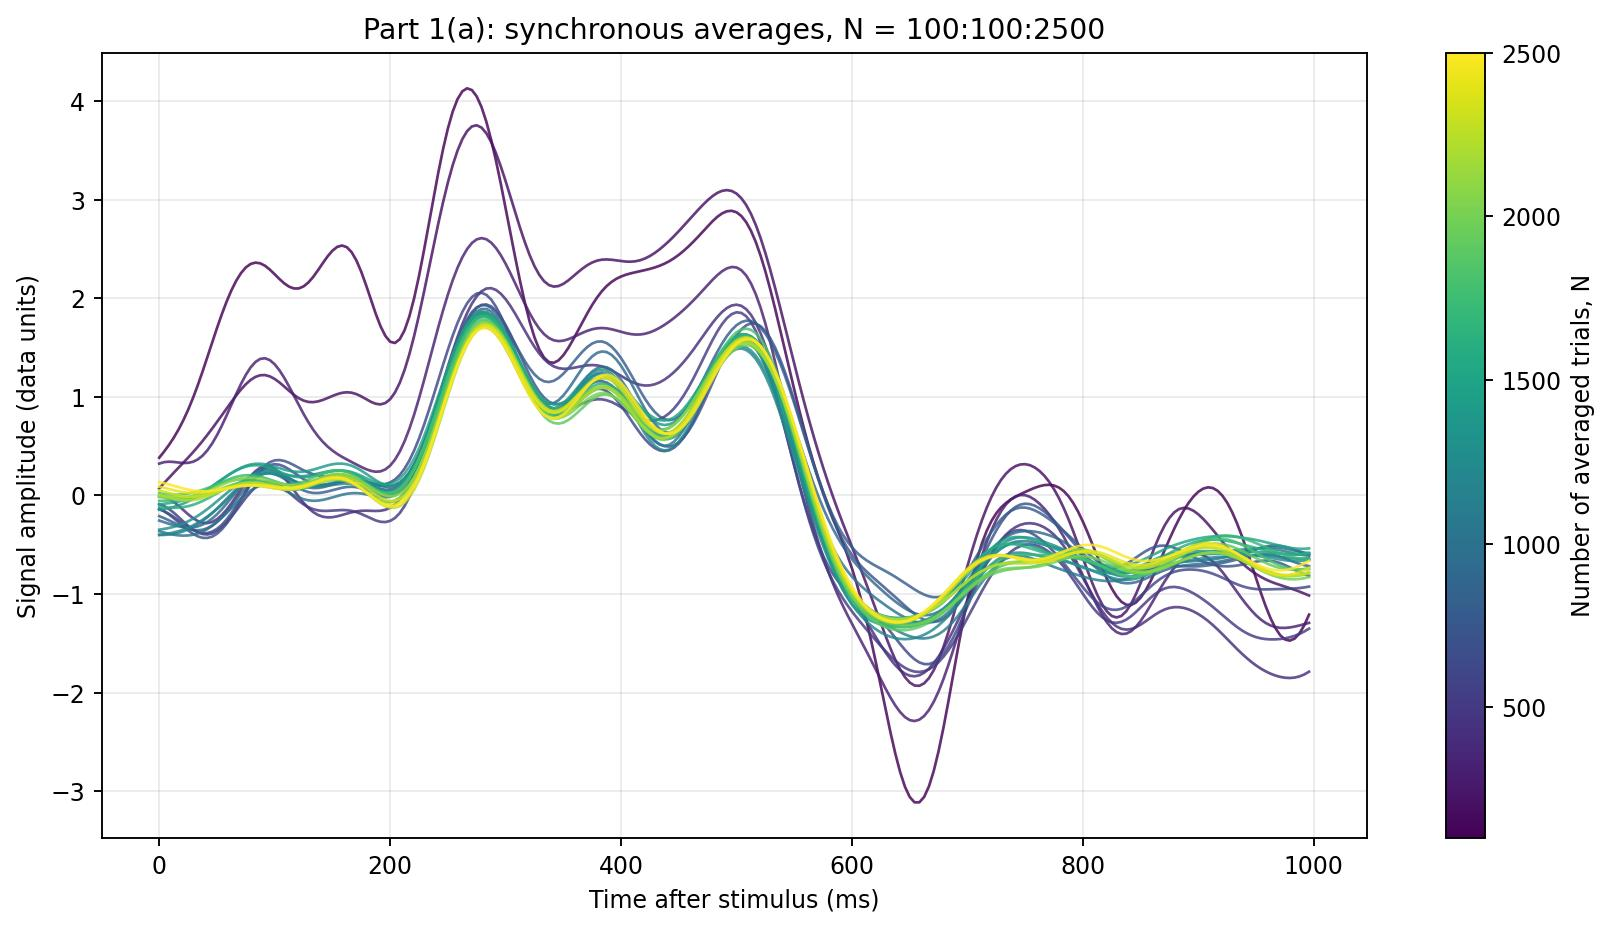
\includegraphics[width=0.95\textwidth]{fig01_p300_averages_n100_to_n2500.png}
\caption{Synchronous average for $N$ from 100 to 2500 in steps of 100; the color of each curve indicates the number of repetitions.}
\label{fig:p300avg}
\end{figure}

\subsection*{(b) and (c) Indices of the change of the average response}
\begin{taskbox}
\textbf{(b)} For $N=1{:}2550$, plot the maximum absolute amplitude of the signal versus the number of averaged patterns in a single graph.\\
\textbf{(c)} Plot the root mean square (RMS) error between the $N$-th average pattern and the $(N-1)$-th average pattern versus the number of averaged patterns $N=1{:}2550$ in a single graph.
\end{taskbox}

\paragraph{(b) Maximum absolute amplitude.} For each number of repetitions, the maximum absolute value of the average response was computed. This value is 10.3790 for one repetition, 4.1276 for 100 repetitions, 2.1013 for 400 repetitions, 1.7106 for 1200 repetitions, and 1.6785 for 2550 repetitions. The overall trend is decreasing, but adding one repetition can cause a local increase or decrease.
\begin{equation}
A_N=\max_k\,|M_N[k]|
\end{equation}

\begin{figure}[H]
\centering
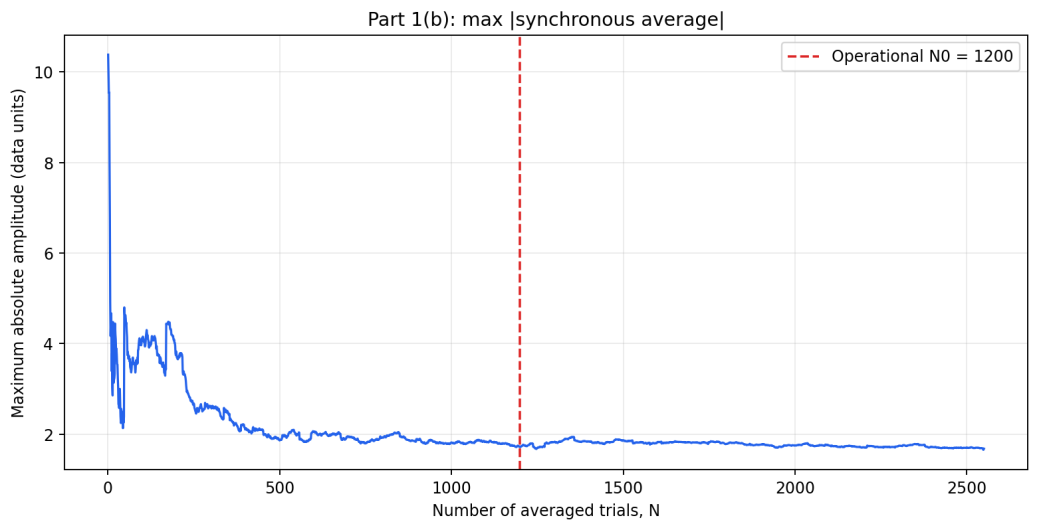
\includegraphics[width=0.85\textwidth]{fig02_max_abs_amplitude_vs_n.png}
\caption{Maximum absolute value of the average response versus the number of repetitions.}
\label{fig:maxabs}
\end{figure}

\paragraph{(c) Differences of successive averages.} The root mean square of the difference between two successive average responses was computed. For $N$ equal to one this quantity is not defined, and it was stored as NaN. Its values at 100, 400 and 1200 repetitions are 0.14025, 0.02364 and 0.00588, respectively. The decreasing trend is consistent with stability; nevertheless, the difference between averages is inherently divided by $N$, and its becoming small does not by itself prove the detection of P300.
\begin{equation}
E_N=\mathrm{RMS}\!\left(M_N-M_{N-1}\right);\qquad N\ge 2
\end{equation}

\begin{figure}[H]
\centering
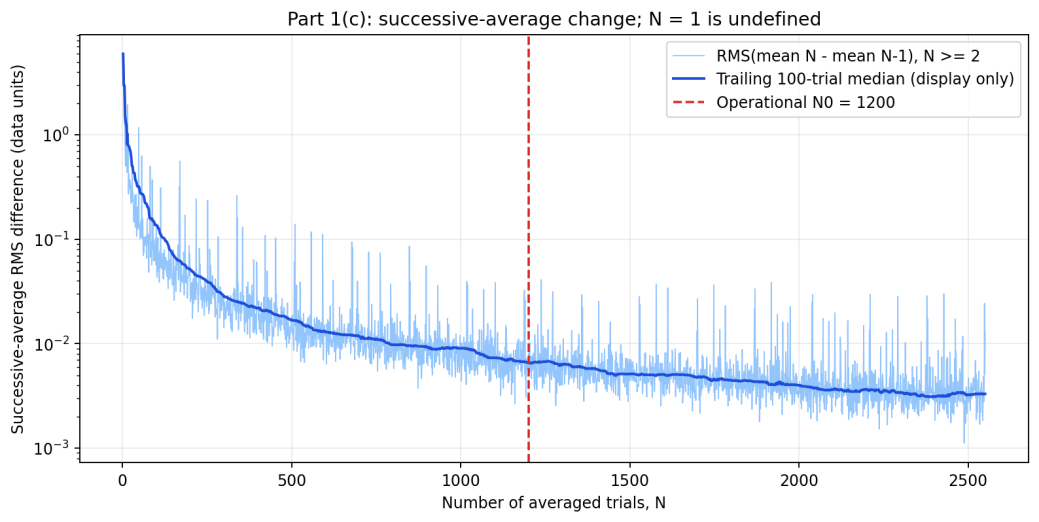
\includegraphics[width=0.85\textwidth]{fig03_rms_difference_consecutive_averages.png}
\caption{RMS difference of successive averages; the vertical axis is logarithmic and the value $N=1$ is undefined.}
\label{fig:rmsdiff}
\end{figure}

\subsection*{(d) Determining the selected number of repetitions}
\begin{taskbox}
Using the results obtained in parts (a), (b) and (c), what is the required number of trials from which the P300 response can be extracted? (Call the obtained number $N_0$.)
\end{taskbox}

The exercise statement did not set a specific numerical threshold for the appearance of the response; we therefore determined the required number of repetitions with an operational criterion for waveform stability. The responses were checked at intervals of 100 repetitions. At each checkpoint, two conditions were required. First, the range of variation of the maximum absolute amplitude of the response in the last 100 repetitions, relative to the median of the same quantity in that interval, is at most 10 percent. Second, the median of the RMS difference of successive averages in the same interval, relative to the maximum absolute response at the checkpoint, is at most one percent. After both conditions held simultaneously at three consecutive checkpoints, the number 1200 repetitions was chosen, and its waveform was also compared with the responses obtained from larger numbers.

This number is neither a unique physiological minimum nor a significance test. For example, by lowering the amplitude-fluctuation threshold to 5 percent, $N_0$ reaches 1900; with a threshold of 15 percent, keeping the one-percent RMS limit, the value 700 is obtained. The number 1200 must therefore be reported together with the definition of the criterion.

\begin{figure}[H]
\centering
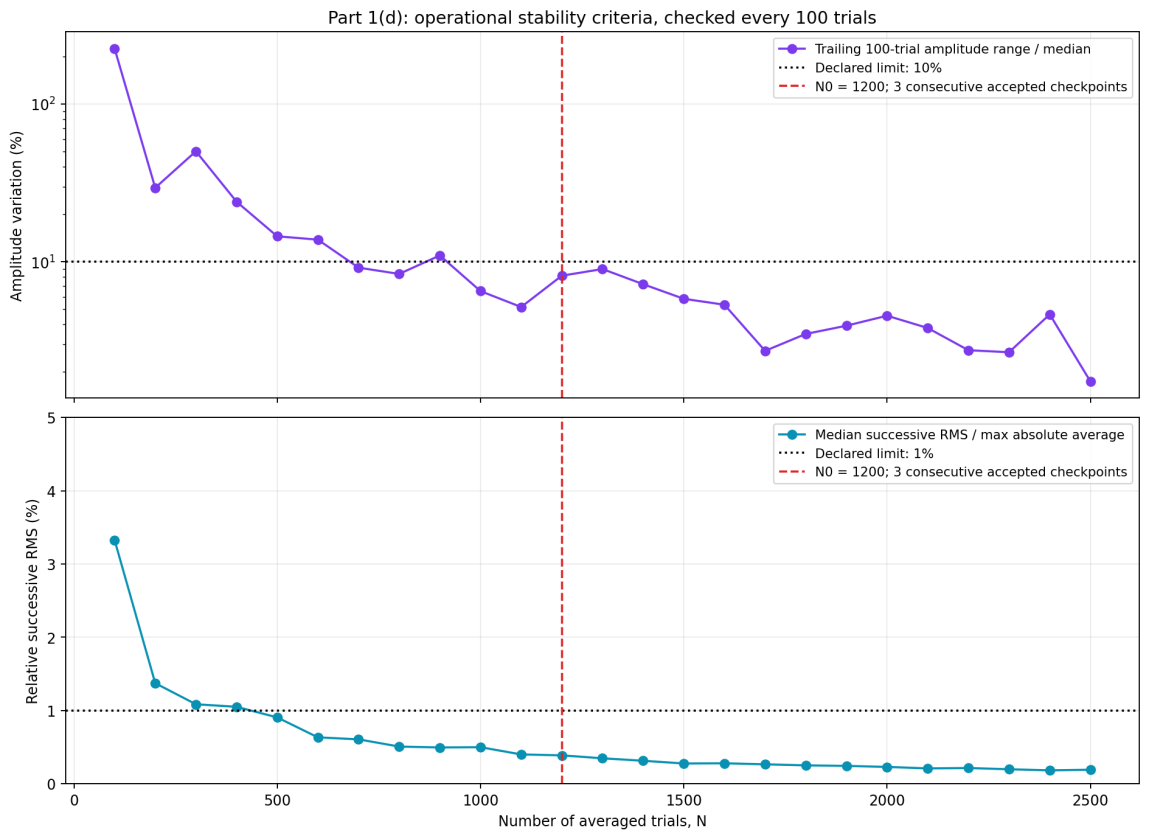
\includegraphics[width=0.85\textwidth]{fig04_stability_criteria_n0.png}
\caption{The two stability criteria and the confirmation point of three consecutive checks at $N_0=1200$.}
\label{fig:stability}
\end{figure}

\begin{table}[H]
\centering
\caption{Sensitivity of the selected number to the amplitude stability threshold, with three consecutive checks held fixed.}
\begin{tabular}{@{}ccc@{}}
\toprule
\textbf{Amplitude-change threshold} & \textbf{Relative RMS threshold} & $N_0$\\
\midrule
5\%  & 1\% & 1900\\
10\% & 1\% & 1200\\
15\% & 1\% & 700\\
\bottomrule
\end{tabular}
\end{table}

\subsection*{(e) Comparison of the number of repetitions and the way of selection}
\begin{taskbox}
In a single graph, plot the average response obtained in part (d) together with the following average responses, and compare them. Examine and analyze the obtained results: the average response for $N=2550$; for $N=N_0/3$; for $N=N_0$ with $N_0$ randomly chosen responses out of the 2550 responses; and for $N=N_0/3$ with $N_0/3$ randomly chosen responses out of the 2550 responses.
\end{taskbox}

The average of the first 1200 repetitions was compared with the average of all 2550 repetitions, the first 400 repetitions, 1200 random repetitions and 400 random repetitions. The random selections were made with seed 42 and without replacement. For the descriptive comparison, the average of all repetitions was taken as the reference.

\begin{figure}[H]
\centering
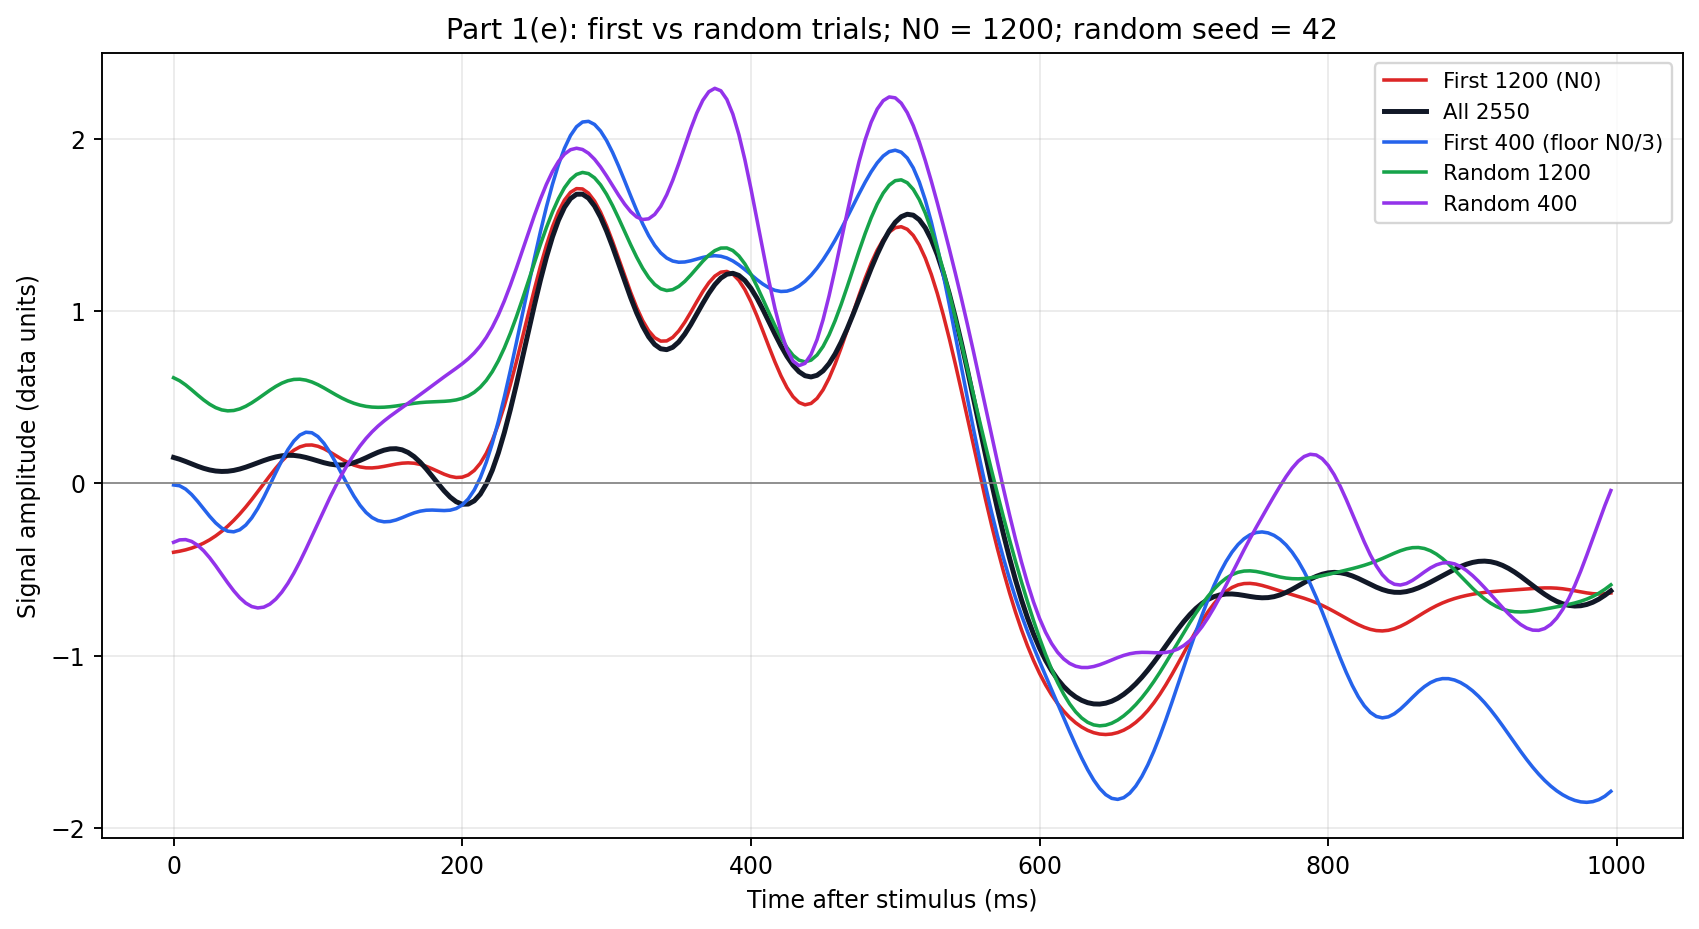
\includegraphics[width=0.85\textwidth]{fig05_comparison_of_five_averages.png}
\caption{Comparison of the five requested responses; the average of all 2550 repetitions is marked with a black line.}
\label{fig:fiveavg}
\end{figure}

\begin{table}[H]
\centering
\caption{Descriptive indices relative to the average of all repetitions; the positive peak is reported in the interval 200 to 600~ms.}
\begin{tabular}{@{}lcccc@{}}
\toprule
\textbf{Response} & \textbf{Positive peak} & \textbf{Latency (ms)} & \textbf{RMS difference} & \textbf{Correlation}\\
\midrule
First 1200 & 1.7106 & 279.17 & 0.1660 & 0.9872\\
All 2550   & 1.6785 & 283.33 & 0.0000 & 1.0000\\
First 400  & 2.1013 & 287.50 & 0.4924 & 0.9551\\
Random 1200 & 1.8046 & 283.33 & 0.2534 & 0.9802\\
Random 400 & 2.2928 & 375.00 & 0.4980 & 0.9193\\
\bottomrule
\end{tabular}
\end{table}

With this specific selection, both 1200-repetition averages are closer to the overall reference than the 400-repetition averages. Random selection has not necessarily made the result better; in this same run, the first 1200 repetitions are closer to the reference than the random sample of 1200 repetitions. The result of one sampling cannot be generalized to all random selections. Moreover, the overall reference itself contains noise and includes the compared repetitions; these indices therefore do not constitute an independent validation.

\subsection*{(f) The number of repetitions in real P300 applications}
\begin{taskbox}
Investigate a few real experiments based on the P300 signal. In real experiments that use P300 patterns (such as P300-based brain-computer interfaces), how many repetitions of the P300 pattern are used? Is this number consistent with the results obtained in the previous parts? Explain the reason for this difference.
\end{taskbox}

In applied studies, a ``repetition'' may refer to the number of sequences, the number of stimulus flashes, or the number of target events. In a $6\times6$ row-column keyboard, one sequence consists of 12 flashes, and the target letter is flashed twice, once with its row and once with its column. Fifteen sequences are therefore equivalent to 180 flashes in total and 30 target events. This unit differs from each single-event column of the file of this exercise.

Lu et al.\ in 2013 used 15 complete sequences for each letter. In the study of Nijboer et al.\ in 2008, the first phase consisted of 20 sequences for each letter, and in the second phase the number of sequences for four participants was chosen as 14, 13, 7 and 4, respectively. Townsend et al.\ in 2010 used five sequences in calibration and adjusted the number of sequences of the online test for each person. The numbers in these examples are usually smaller than $N_0$ of this exercise, but the aim of a practical system is target selection with multichannel features and a trained classifier; this exercise examines the stability of the waveform of a single channel with averaging. The difference in the unit of repetition, the amount of noise, the person's attention, the timing of the stimuli and the success criterion limits a direct comparison of the numbers. No universal minimum for the required number can be derived from these papers.

\begin{table}[H]
\centering
\caption{Applied examples; the number of sequences is not the same as the number of single-event responses of the exercise.}
\begin{tabularx}{\textwidth}{@{}>{\raggedright\arraybackslash}p{3.1cm}>{\raggedright\arraybackslash}X>{\raggedright\arraybackslash}X@{}}
\toprule
\textbf{Study} & \textbf{Sequence protocol} & \textbf{Target events}\\
\midrule
Lu et al.\ 2013 & 15 sequences of 12 stimuli per letter & 30 target events; 180 flashes in total\\
Nijboer et al.\ 2008 & 20 sequences in the first phase; 4 to 14 in the second phase & 40 target events in the first phase\\
Townsend et al.\ 2010 & 5 calibration sequences; individual adjustment in the test & 10 target events in calibration\\
\bottomrule
\end{tabularx}
\end{table}

This difference does not prove an inconsistency between the result of the exercise and practical application. To reveal a stable waveform, a criterion different from that of selecting one letter correctly with a multichannel classifier was used. The appropriate number of repetitions must be reported together with the counting unit, the recording conditions and the decision criterion.

\section{Part 2: SSVEP Analysis}

\begin{taskbox}[Part 2: introduction in the lab manual]
The file \texttt{SSVEP\_EEG.mat} contains the SSVEP signal recorded from one user. This file contains a matrix \texttt{SSVEP\_Signal} (EEG recorded from 6 channels Pz, Oz, P7, P8, O1 and O2, with sampling frequency 250 Hz), a matrix \texttt{Events} (stimulation frequencies) and a matrix \texttt{Event\_Samples} (the time sample corresponding to the start of each stimulus). The goal is to determine the stimulation frequency from the EEG signal recorded in each trial.
\end{taskbox}

\subsection*{(a) Data and band-pass filter}
\begin{taskbox}
For each channel of the data, use a band-pass filter to remove the frequencies below 1 Hz and above 40 Hz. For each channel, plot the denoised signal together with the original signal in one graph.
\end{taskbox}

The SSVEP signal consists of six channels, Pz, Oz, P7, P8, O1 and O2, sampled at 250~Hz. For 15 stimuli, the goal is to detect the fundamental stimulation frequency from the EEG and to examine the differences between the responses of the channels. Five frequencies, 6.5, 7.35, 8.3, 9.6 and 11.61~Hz, were each recorded three times. According to the basis of the lab notes, the SSVEP response can have components at the stimulation frequency and at its integer multiples.

For each of the six channels, a Butterworth band-pass filter with cutoffs of 1 and 40~Hz, implemented with second-order sections, was designed. The order of the initial prototype is four, and the final band-pass order is eight in each pass. The filter was applied forward and backward on the continuous signal so as not to create phase delay in the offline analysis; in this case the amplitude response equals the square of the amplitude response of the single pass. Filtering before cutting the repetitions prevents a separate transient at the beginning of each repetition.

The comparison of the raw and the filtered recording shows the removal of most of the slow trend and of the out-of-band variations. A real filter has a gradual transition; cutoffs of 1 and 40~Hz do not mean an ideal, sudden removal of all power outside this range.

\begin{figure}[H]
\centering
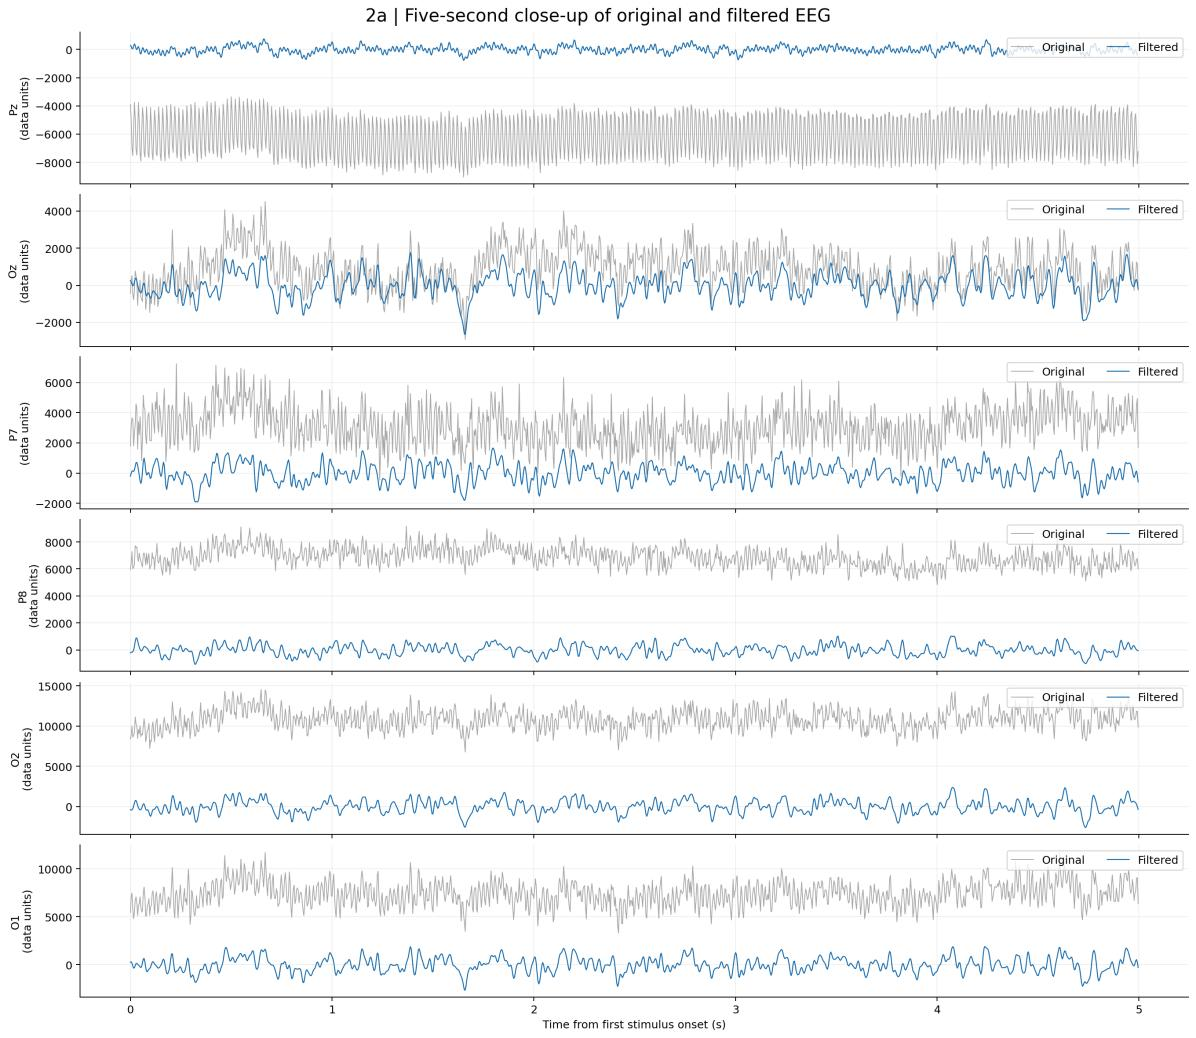
\includegraphics[width=0.9\textwidth]{fig06_ssvep_bandpass_filter_check.png}
\caption{The original signal and the output of the 1 to 40~Hz filter in the first five seconds of the first stimulus, for all six channels.}
\label{fig:ssvepfilter}
\end{figure}

\subsection*{(b) and (c) Windowing and spectrum estimation}
\begin{taskbox}
\textbf{(b)} Extract the 15 trials corresponding to the 15 stimuli, each with a 5-second window.\\
\textbf{(c)} For each trial, compute the frequency content of all six channels and plot them in one figure. You can use the function \texttt{pwelch}. Use an appropriate legend to indicate which channel each curve belongs to.
\end{taskbox}

\paragraph{(b) Separating the fifteen repetitions.} The start index of each stimulus was read from the variable \texttt{Event\_Samples}. Since MATLAB's index starts from one and Python's from zero, one unit was subtracted from each number. From the start of each stimulus, exactly five seconds, or 1250 samples, were taken. The final array has dimensions 15 repetitions $\times$ 6 channels $\times$ 1250 samples, and the completeness of all windows was checked.

\paragraph{(c) Computing the power spectral density.} The power spectral density of each channel in each repetition was computed with Welch's method. A Hann window of 625 samples, an overlap of 312 samples and an FFT length of 4096 were used. The basic frequency spacing corresponding to the segment length, $f_s/L$, is 0.4~Hz; the true resolving power also depends on the window shape. Zero-padding makes the display grid finer, with a spacing of about 0.061~Hz, but it does not increase the true resolution of the information. For each repetition, the six spectra are drawn in one figure with a legend of channel names; in addition to 15 separate figures, a collective view was also prepared.

The fifteen six-channel spectra are given separately in Appendix~A. The sample display of channel Oz in the figure below shows that the lengths of the windows are identical and that the time starts from the moment of the stimulus.

\begin{figure}[H]
\centering
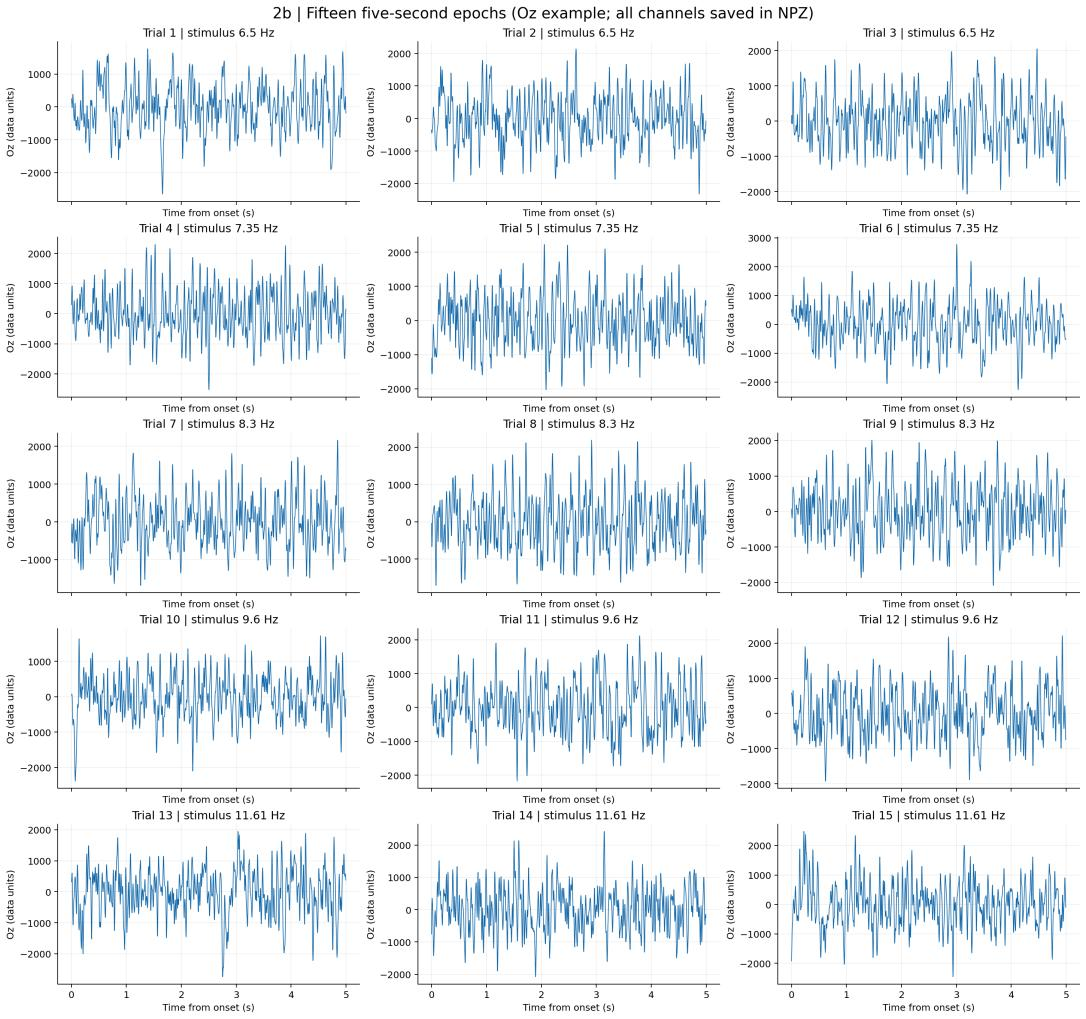
\includegraphics[width=0.9\textwidth]{fig07_ssvep_fifteen_windows_oz.png}
\caption{The fifteen five-second windows; channel Oz was chosen for display, and the spectral analysis was performed on all six channels.}
\label{fig:ssvepwin}
\end{figure}

\subsection*{(d) and (e) Differences between the channels and detection of the frequency}
\begin{taskbox}
\textbf{(d)} For a single trial, do all channels have the same frequency content? What is the reason for the differences in the frequency content of the channels?\\
\textbf{(e)} For each trial, can you determine the dominant frequency using the frequency content of the channels? To which frequencies do the spectral peaks correspond? Why does each of these peaks arise?
\end{taskbox}

\paragraph{(d) Comparison of the channels.} The spectra of the six channels are not identical in amplitude and shape. In this data, the mean power at the target frequency in the posterior channels Oz, O1 and O2 is higher than in Pz. The electrode location, the combination of sources and volume conduction, electrode noise and the background EEG can play a role in this difference; the present data do not determine the physiological cause of each difference conclusively.

\paragraph{(e) Fundamental frequency and harmonics.} To avoid mistaking slow background activity for the stimulation frequency, the simple search for the highest peak was explicitly performed in the range of 5 to 40~Hz. In 8 of the 15 repetitions, this peak is near the second harmonic of the stimulus. For the 6.5 and 7.35~Hz stimuli, the dominant peaks are seen at about 13 and 14.7~Hz, respectively. In the 8.3~Hz group, two repetitions have a dominant peak near 16.6~Hz and one repetition has a dominant peak near the fundamental frequency. In the 9.6 and 11.61~Hz groups, the dominant peak is mainly near the fundamental frequency. The highest peak of the spectrum is therefore not necessarily the stimulation frequency itself.

Peaks at multiples can arise from the non-sinusoidal shape of the response or from the nonlinearity of the visual pathway. Other peaks may also be related to the background EEG, alpha activity, artifacts or spectral leakage. Comparing the power at the five permitted fundamental frequencies gave the correct answer in all 15 repetitions.

\begin{table}[H]
\centering
\caption{The peak was searched for in the range of 5 to 40~Hz; the output of the PSD at the permitted fundamental frequencies and of CCA is identical in all 15 rows.}
\begin{tabular}{@{}cccc@{}}
\toprule
\textbf{Repetition} & \textbf{Stimulus (Hz)} & \textbf{Highest peak (Hz)} & \textbf{Estimate of both methods (Hz)}\\
\midrule
1  & 6.5   & 12.939 & 6.5\\
2  & 6.5   & 12.939 & 6.5\\
3  & 6.5   & 13.062 & 6.5\\
4  & 7.35  & 14.648 & 7.35\\
5  & 7.35  & 14.648 & 7.35\\
6  & 7.35  & 14.648 & 7.35\\
7  & 8.3   & 16.541 & 8.3\\
8  & 8.3   & 8.362  & 8.3\\
9  & 8.3   & 16.663 & 8.3\\
10 & 9.6   & 9.521  & 9.6\\
11 & 9.6   & 9.705  & 9.6\\
12 & 9.6   & 9.644  & 9.6\\
13 & 11.61 & 11.658 & 11.61\\
14 & 11.61 & 11.536 & 11.61\\
15 & 11.61 & 11.597 & 11.61\\
\bottomrule
\end{tabular}
\end{table}

\subsection*{(f) A complementary multichannel method}
\begin{taskbox}
Do you know another method for determining the dominant frequency in the SSVEP signal that gives better results than using the frequency content of the individual channels? By searching the internet and relevant papers, name other methods for processing SSVEP signals and determining the dominant frequency.
\end{taskbox}

Canonical correlation analysis (CCA) compares a linear combination of the EEG channels with a linear combination of sine and cosine references. For each candidate frequency, a reference of the fundamental frequency and of the second and third harmonics was built. The largest canonical correlation is the score of the candidate, and the largest score determines the predicted frequency. The references are built identically for all five candidates; the true label of a repetition is not used in selecting the answer, and only the set of the permitted frequencies of the system is assumed known. Lin et al.\ introduced this approach for SSVEP detection in 2006.
\begin{equation}
\rho(f)=\max\operatorname{corr}(Xw,\,Y_f v);\qquad
\hat f=\arg\max_f\rho(f)
\end{equation}

CCA can use the joint temporal and spatial information of several channels. The FBCCA method, introduced by Chen et al.\ in 2015, combines the information of the bands and harmonics with a filter bank. TRCA, introduced by Nakanishi et al.\ in 2018, uses labeled training repetitions to learn a spatial filter and an individual template. In this exercise, the complementary method that was run is ordinary CCA; FBCCA and TRCA are introduced only as a research answer.

CCA gave 15 correct answers in the same 15 repetitions. Since the PSD baseline at the permitted candidates also has 15 correct answers, a numerical superiority of CCA was not observed in this sample. In addition, this accuracy is descriptive, obtained from one person and 15 repetitions, and is not an estimate of performance on independent persons or data.

\begin{figure}[H]
\centering
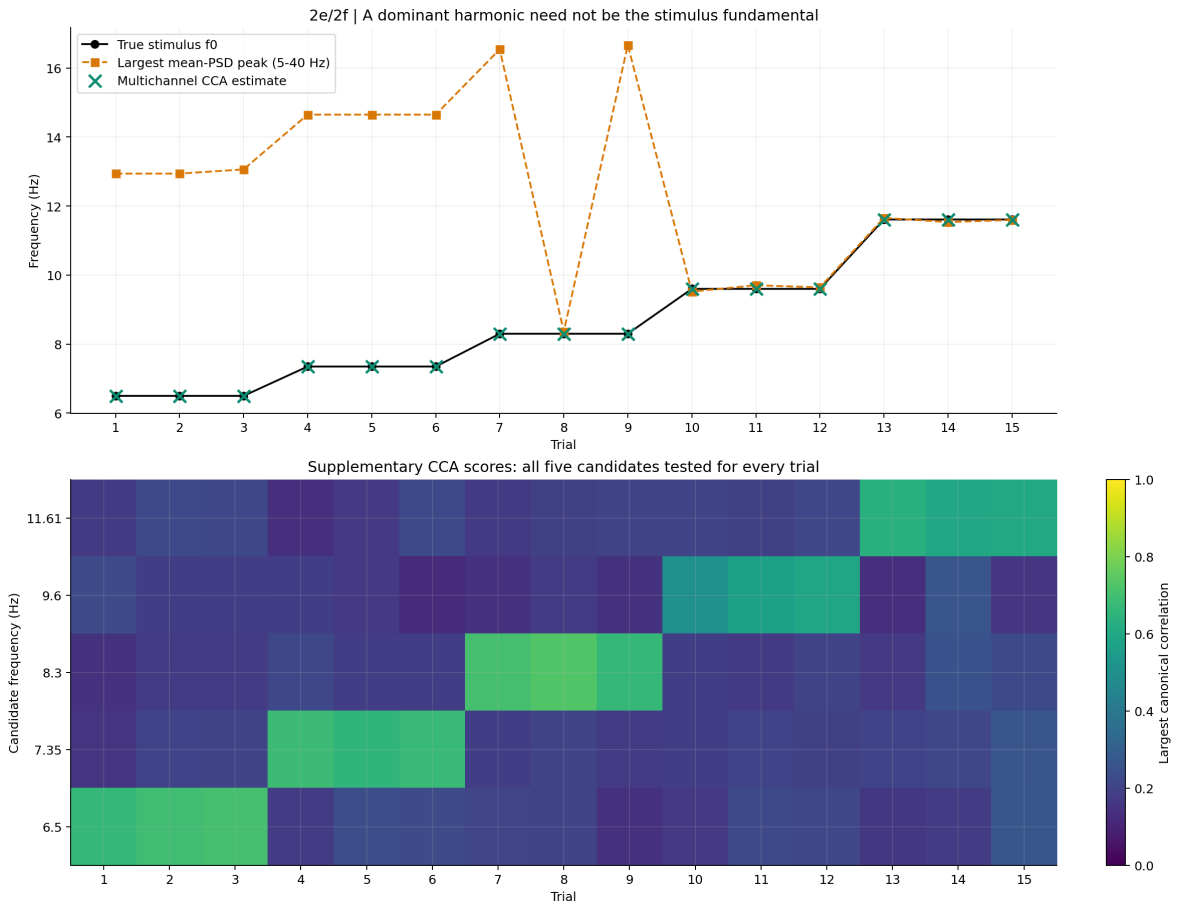
\includegraphics[width=0.8\textwidth]{fig08_ssvep_frequency_estimates.png}
\caption{Comparison of the true frequency, the highest peak and the CCA estimate; below, the score of all five candidates in each repetition is shown.}
\label{fig:ccaest}
\end{figure}

\section{Part 3: Examination of ERD and ERS}

\begin{taskbox}[Part 3: introduction in the lab manual]
The file \texttt{FiveClass\_EEG.mat} contains an EEG signal recorded at a sampling frequency of 256 Hz from one user while performing different mental tasks, from 30 channels of the international 10-20 system. Five mental tasks were assigned: (1) word generation, (2) mental subtraction, (3) navigation, (4) hand movement imagery and (5) foot movement imagery. In each trial, a ``+'' sign is first shown (time zero), after 3 seconds a beep is played and the task is shown, and the person performs the task for 7 seconds (until the second beep); between two trials there is a rest of 2.5 to 3.5 seconds. The data contain the matrix \texttt{X} (the recorded EEG), the vector \texttt{y} (the class label of each of the 200 trials) and the vector \texttt{trial} (the sample number of the start of each trial). We want to examine the changes of the signal in different frequency bands in each of the five classes.
\end{taskbox}

\subsection*{Data and task timing}

The continuous data of this part have 714701 samples and 30 channels and were recorded at a rate of 256~Hz. The 200 repetitions are divided into five classes, and each class has 40 repetitions: word generation, mental subtraction, navigation, hand movement imagery and foot movement imagery. Time zero is the display of the concentration cross; the task starts at about the third second and ends at the tenth second. The central channel CPz was chosen for the comparison plots.

\subsection*{(a) Four-band filtering}
\begin{taskbox}
First, filter the signal of each channel in the following four bands: delta (1 to 4 Hz), theta (4 to 8 Hz), alpha (8 to 13 Hz) and beta (13 to 30 Hz). For this purpose you can use the filter given in the manual (a 4th-order Chebyshev type I band-pass filter with 1 dB passband ripple, applied with \texttt{filter}). To make sure the filters work correctly, plot about 5 seconds of the first channel of \texttt{X}, the original signal and the four signals obtained in the different bands.
\end{taskbox}

The continuous signal of each channel was filtered with a type I Chebyshev filter of final order four and a ripple of one decibel. The filter was applied causally, as in the \texttt{filter} command of the experiment statement. In the SciPy implementation, an initial prototype order of two gives a final order of four after the band-pass transformation. The bands, according to the lab manual, are delta 1 to 4, theta 4 to 8, alpha 8 to 13 and beta 13 to 30~Hz.

\begin{figure}[H]
\centering
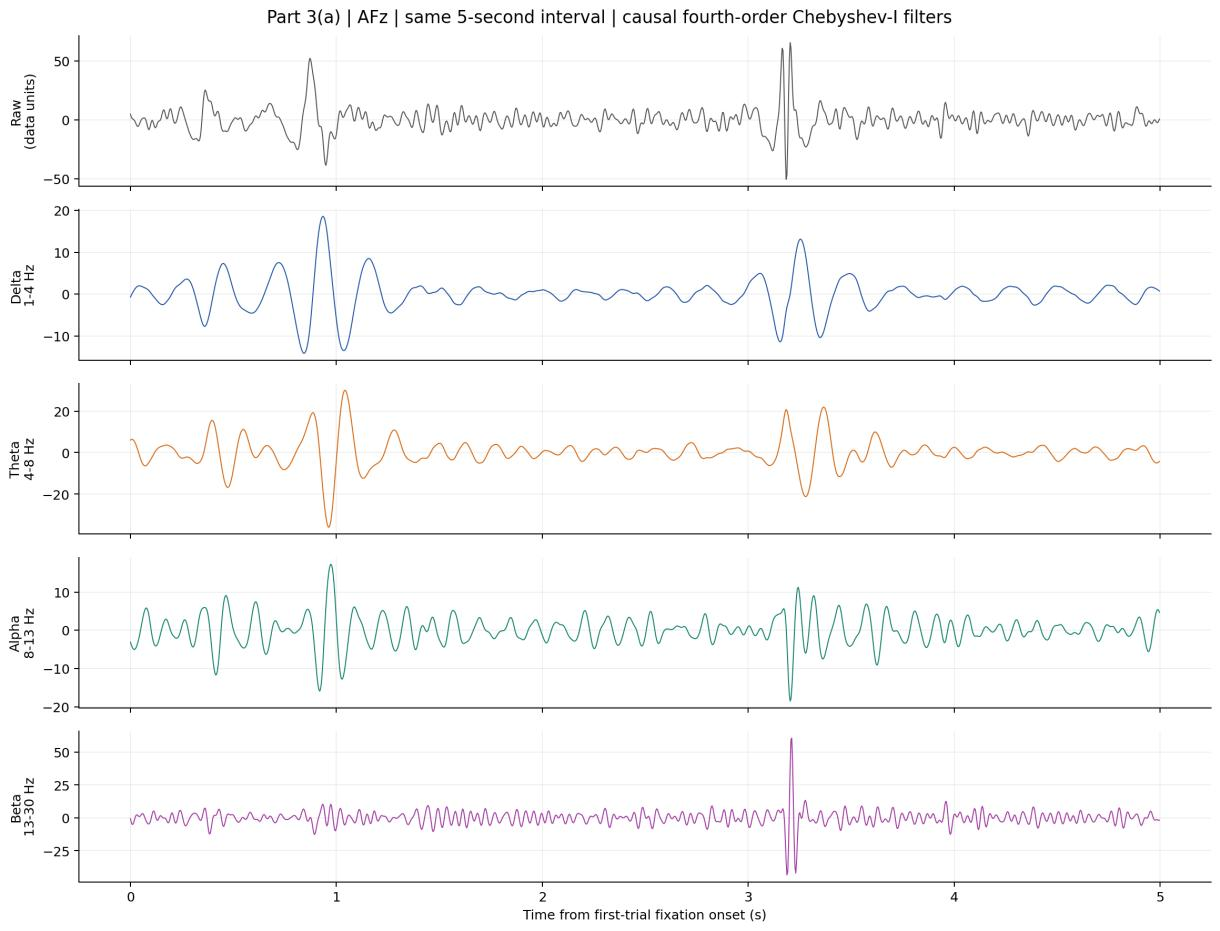
\includegraphics[width=0.9\textwidth]{fig09_erd_filter_check_afz.png}
\caption{The first five seconds of the first repetition in channel AFz; the raw signal and the output of all four bands over the same time interval.}
\label{fig:erdfilter}
\end{figure}

\subsection*{(b) to (e) Computing and smoothing the power}

\paragraph{(b) Separating the ten-second repetitions.}
\begin{taskbox}
Extract the 10-second trials from the obtained signals (using the information in the vector \texttt{trial}).
\end{taskbox}
After converting the start index, exactly 2560 samples were taken from each repetition. The tensor of each band therefore has dimensions 2560 samples $\times$ 30 channels $\times$ 200 repetitions. The index range of the MATLAB code in the PDF creates 2561 samples because it includes both ends; in this analysis the length of 2560 samples explicitly requested in the output dimensions was respected.

\paragraph{(c) and (d) Squared amplitude and the mean of each class.}
\begin{taskbox}
\textbf{(c)} To compute the power at each point, compute the square of the amplitude of all time points for each trial in each band and each channel.\\
\textbf{(d)} According to the labels of the 200 trials (in the vector \texttt{y}), separate the data of the 5 different classes and, for each band, obtain the mean of each channel over the trials of that class. The output is four tensors of size $2560\times30\times5$ (\texttt{Delta\_X\_avg}, \texttt{Theta\_X\_avg}, \texttt{Alpha\_X\_avg}, \texttt{Beta\_X\_avg}), where 30 is the number of channels and 5 the number of classes.
\end{taskbox}
The amplitude of all samples, in each repetition and each channel, was first squared. Then, with the label $y$, the power of the repetitions of each class was averaged. The output of each band is a tensor of $2560\times30\times5$. This order preserves the power of oscillations that have no phase locking, and it is consistent with the method of the lecture notes.
\begin{align}
p_{i,b,c}[k]&=\bigl(x_{i,b,c}[k]\bigr)^{2}\\
P_{j,b,c}[k]&=\frac{1}{n_j}\sum_{i\in I_j}p_{i,b,c}[k];\qquad n_j=40
\end{align}
In the relation above, the set of the indices of the repetitions of each class is shown with a subscripted symbol. The number of members of this set is 40 in each of the five classes.

\paragraph{(e) Temporal smoothing.}
\begin{taskbox}
To smooth the variations in the average signals of part (d), filter the signal of each channel in each of the trials and in each band using a rectangular window defined as \texttt{newWin = ones(1,200)/sqrt(200)} and the \texttt{conv} command.
\end{taskbox}
A rectangular window was built exactly according to the problem statement, with 200 coefficients equal to one over the square root of 200. The sum of the coefficients is 14.142; its output is therefore 14.142 times the conventional moving average with coefficients of one over 200. This scale is stated on the axis of the power plots. The convolution was performed in the \texttt{same} mode so that the time axis remains ten seconds.
\begin{equation}
w[k]=\frac{1}{\sqrt{200}}\qquad\text{for } 0\le k<200
\end{equation}
This window is about 0.78~s long and is applied centered; the effect of a change can spread to about 0.39~s on either side of it. Zero-padding at the two ends creates an artificial drop; the edge regions are shaded in the plots and were not the basis for interpreting the task changes.

\paragraph{Complementary measurement relative to the baseline.} For a relative comparison, the mean smoothed power in the interval 0.5 to 2.5~s was taken as the baseline of each class and channel. The percentage change was summarized in the interval 3.5 to 9.5~s. In this way, the convolution edges and the transition at the task onset were avoided. The constant coefficient of the window cancels in the following ratio; a negative sign is ERD and a positive sign is ERS.
\begin{equation}
\mathrm{ERD/ERS}[k]=100\times\frac{P[k]-R}{R}
\end{equation}

\subsection*{(f) Delta and theta band power at CPz}
\begin{taskbox}
Choose one channel (preferably a channel from the central regions of the head, such as CPz) and plot the results of part (e) for it: for each frequency band, plot the time-averaged signal (over the 10-second interval) of all 5 classes in one figure (four figures in total, with 5 curves in each figure).
\end{taskbox}

In each figure, the smoothed mean-power curves of the five classes are shown. The dashed line is the beginning of the task at the third second. The blue region is the baseline interval of the relative analysis, and the gray regions show the two convolution edges.

\begin{figure}[H]
\centering
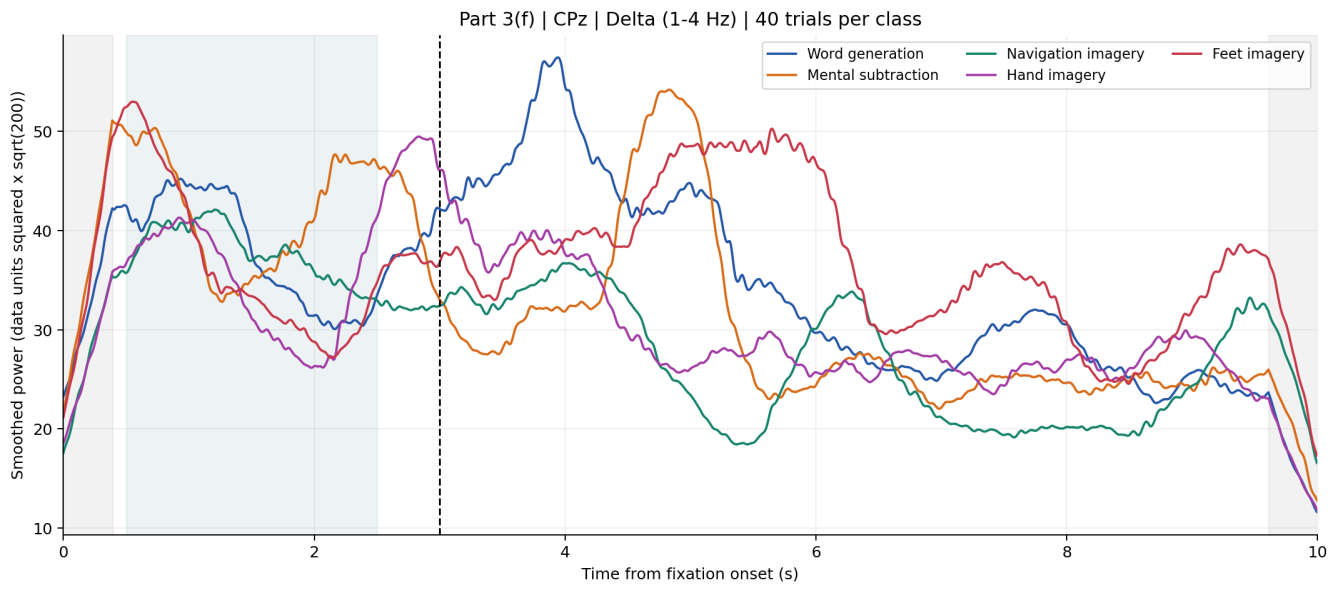
\includegraphics[width=0.85\textwidth]{fig10_delta_power_five_classes.png}
\caption{Smoothed delta power (1 to 4~Hz) in the five classes.}
\label{fig:delta}
\end{figure}

\begin{figure}[H]
\centering
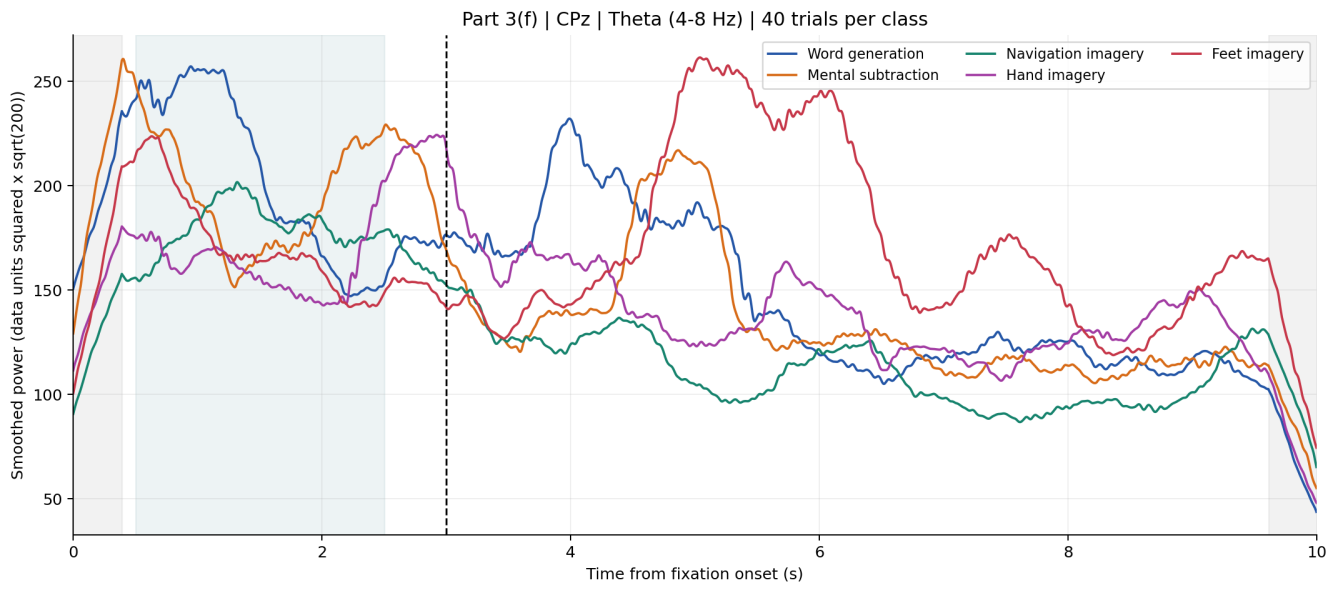
\includegraphics[width=0.85\textwidth]{fig11_theta_power_five_classes.png}
\caption{Smoothed theta power (4 to 8~Hz) in the five classes.}
\label{fig:theta}
\end{figure}

At CPz, navigation and subtraction show a decrease in delta and theta power over most of the activity interval. Foot imagery shows an increase in power in part of the interval. For comparing the classes, the difference in baseline power must also be taken into account; the size of the relative change cannot be concluded from the absolute height of the curves alone.

\subsection*{(f, continued) Alpha and beta band power at CPz}

\begin{figure}[H]
\centering
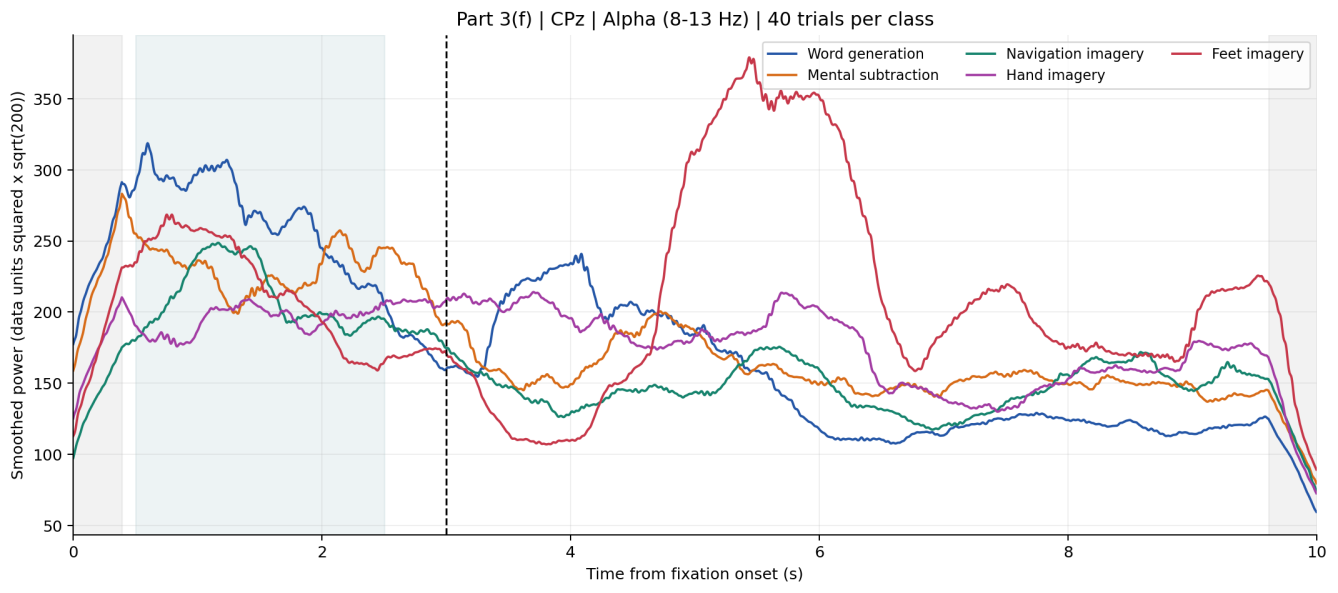
\includegraphics[width=0.85\textwidth]{fig12_alpha_power_five_classes.png}
\caption{Smoothed alpha power (8 to 13~Hz) in the five classes.}
\label{fig:alpha}
\end{figure}

\begin{figure}[H]
\centering
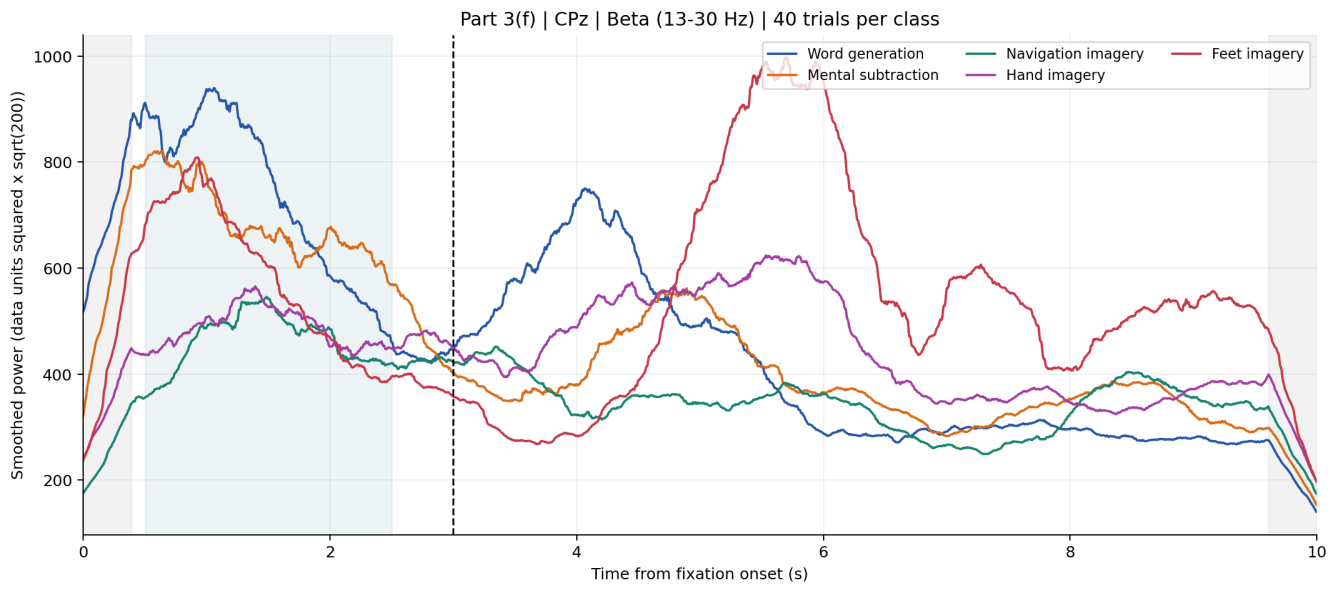
\includegraphics[width=0.85\textwidth]{fig13_beta_power_five_classes.png}
\caption{Smoothed beta power (13 to 30~Hz) in the five classes.}
\label{fig:beta}
\end{figure}

Word generation in this channel, especially in the second half of the task, shows a more definite decrease in alpha and beta. Foot imagery has a transient increase near the fifth and sixth seconds and then decreases; a single temporal average therefore does not reflect all the details of the trend. Hand imagery has smaller average changes than word generation and subtraction.

\subsection*{(g) Interpretation of the relative power changes}
\begin{taskbox}
Considering that the mental tasks start at approximately the third second, by comparing the plots obtained in part (f), what conclusions can be drawn about the frequency information of the five classes?
\end{taskbox}

\begin{table}[H]
\centering
\caption{Mean percentage change of the smoothed power at CPz during 3.5 to 9.5~s relative to the baseline of 0.5 to 2.5~s.}
\begin{tabular}{@{}lrrrr@{}}
\toprule
\textbf{Class} & \textbf{Delta (\%)} & \textbf{Theta (\%)} & \textbf{Alpha (\%)} & \textbf{Beta (\%)}\\
\midrule
Word generation & $-11.10$ & $-31.15$ & $-44.96$ & $-47.19$\\
Subtraction     & $-29.26$ & $-31.75$ & $-31.93$ & $-44.45$\\
Navigation      & $-32.06$ & $-39.87$ & $-30.93$ & $-27.53$\\
Hand imagery    & $-17.07$ & $-15.59$ & $-11.50$ & $-8.46$\\
Foot imagery    & $+3.18$  & $+1.81$  & $-1.86$  & $-4.53$\\
\bottomrule
\end{tabular}
\end{table}

\begin{figure}[H]
\centering
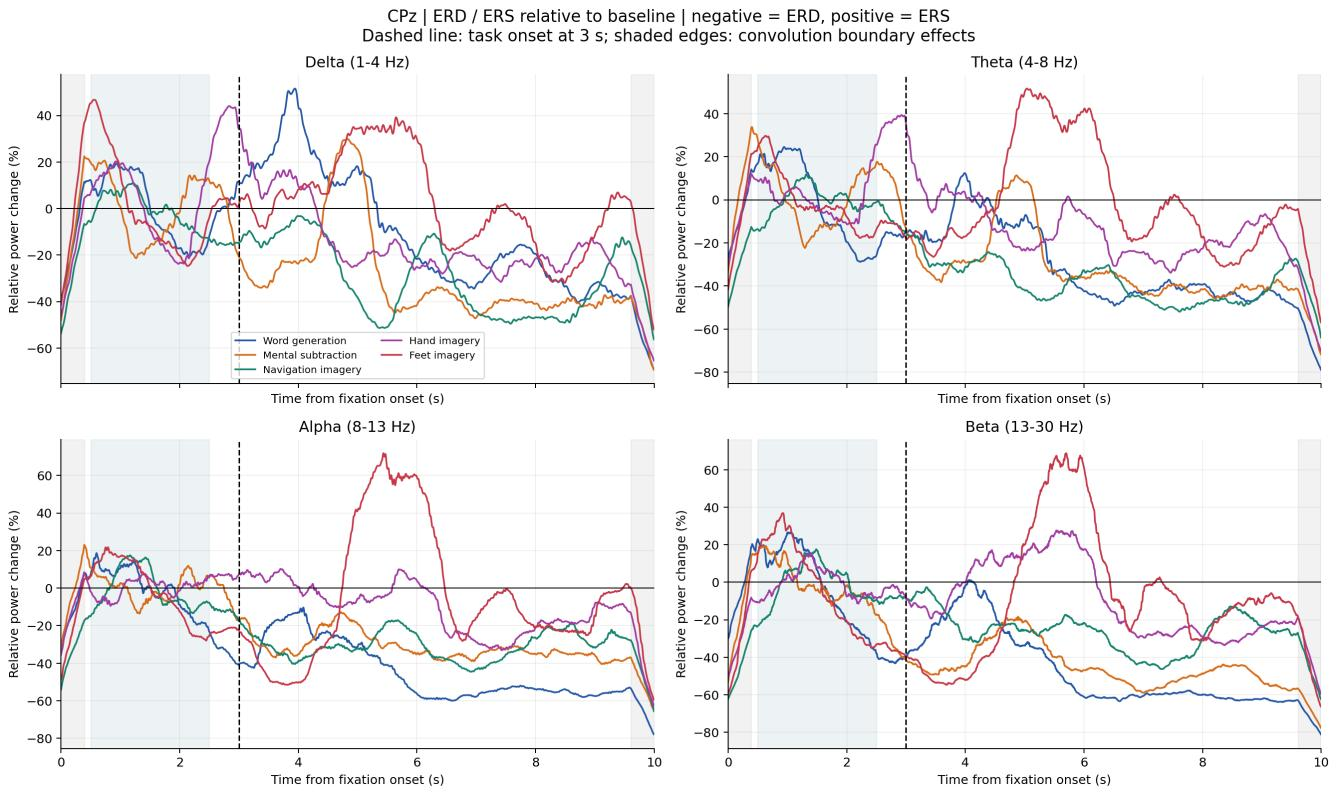
\includegraphics[width=0.85\textwidth]{fig14_relative_trend_four_bands.png}
\caption{Relative trend of the four bands; zero is the baseline power of the same class.}
\label{fig:relative}
\end{figure}

The largest average decrease of alpha and beta belongs to word generation, 44.96 and 47.19 percent, respectively, and the largest decrease of theta belongs to navigation, with 39.87 percent. Foot imagery has a smaller average change: delta and theta are slightly positive, and alpha and beta are slightly negative. This description is limited to channel CPz and the specified intervals and does not mean that there is no relevant activity in the other channels.

The difference between the class means can be a basis for extracting band-power features, but it does not prove the separability of the classes, statistical significance or classification accuracy. The readiness before the task, the delay of the causal filter and the centered smoothing also affect the interpretation of the time at which the changes begin.

\section{Discussion and Conclusions}

\subsection*{Fit of the processing method to the type of response}

The three parts show that the type of time-locking of the response determines the choice of the processing method. For the ERP, synchronous averaging of the voltage is useful; in the SSVEP, the frequency pattern and the harmonics carry the information about the target; and in ERD/ERS, the averaging must be done after computing the power. Treating these three methods as the same can hide an important part of the response.

\subsection*{Main results}

In the first part, the shape of the response became more stable as the number of repetitions increased. The average of the first 1200 repetitions had an RMS difference of 0.1660 and a correlation of 0.9872 relative to the overall average. Given the dependence of $N_0$ on the threshold, a suitable report of the result states the value together with the definition of the stability criterion.

In the second part, both the PSD at the permitted candidates and CCA gave fifteen correct answers. The presence of a dominant second harmonic in eight repetitions showed that detecting the stimulus from the absolute maximum of a spectrum is not sufficient. The label of each repetition was used only after the prediction, for evaluation; the set of the permitted frequencies of the system was assumed known.

In the third part, the patterns of power change of the five tasks at CPz were different. Word generation showed a stronger decrease in alpha and beta, and navigation showed a stronger decrease in theta. The transient increase of foot imagery also showed that analyzing the temporal trend provides more information than a single average number.

\subsection*{Limitations and reproducibility}

The overall ERP average is not a noise-free or independent reference, and it overlaps with the subsets. The SSVEP accuracy was obtained from only fifteen repetitions of one person. In ERD/ERS, no statistical test or classifier was run with independent test data. The present results should therefore be interpreted as a descriptive analysis of these same data.

All analyses were run with Python. The random selection seed is 42. The independent files \texttt{part1\_erp.py}, \texttt{part2\_ssvep.py} and \texttt{part3\_erd\_ers.py} have a Persian comment on every line; the parameters, the CSV results and the NPZ tensors were saved in the solution package. Direct checks of the averages, the slice indices, Welch's method, the tensor dimensions and the CPz convolution matched the saved outputs.

\clearpage
\section*{Appendix A: Spectra of the Six Channels in Each Repetition}

The Welch spectra were drawn with the same data and parameters as in Part~2. The dashed lines show the stimulation frequency and its multiples. The amplitude is in decibels relative to one unit of data squared per hertz.

\begin{figure}[p]
\centering
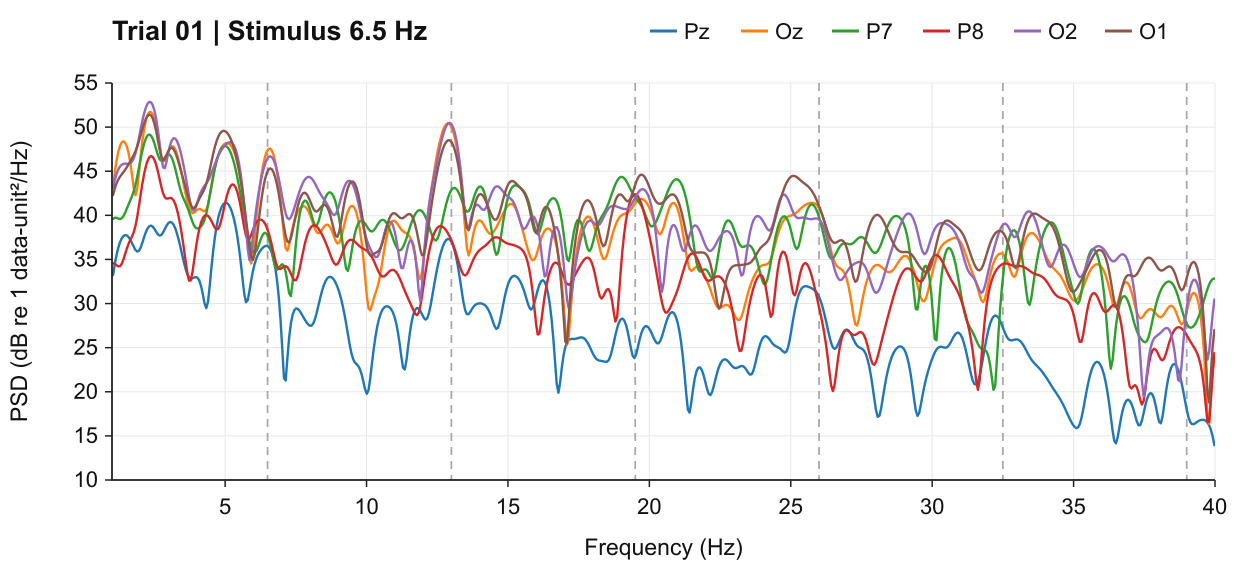
\includegraphics[width=0.9\textwidth,height=0.4\textheight,keepaspectratio]{fig15_ssvep_trial01_6p5hz.png}
\caption{Repetition 1 with a stimulation frequency of 6.5~Hz; all six channels are shown on one axis.}
\label{fig:app15}
\end{figure}

\begin{figure}[p]
\centering
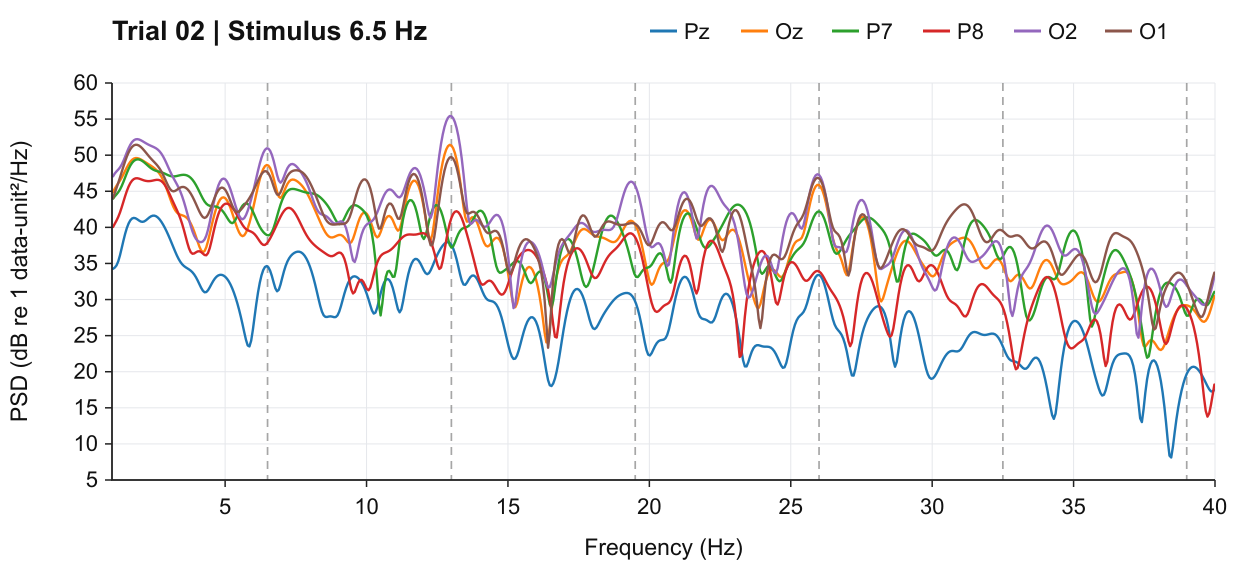
\includegraphics[width=0.9\textwidth,height=0.4\textheight,keepaspectratio]{fig16_ssvep_trial02_6p5hz.png}
\caption{Repetition 2 with a stimulation frequency of 6.5~Hz; all six channels are shown on one axis.}
\label{fig:app16}
\end{figure}

\begin{figure}[p]
\centering
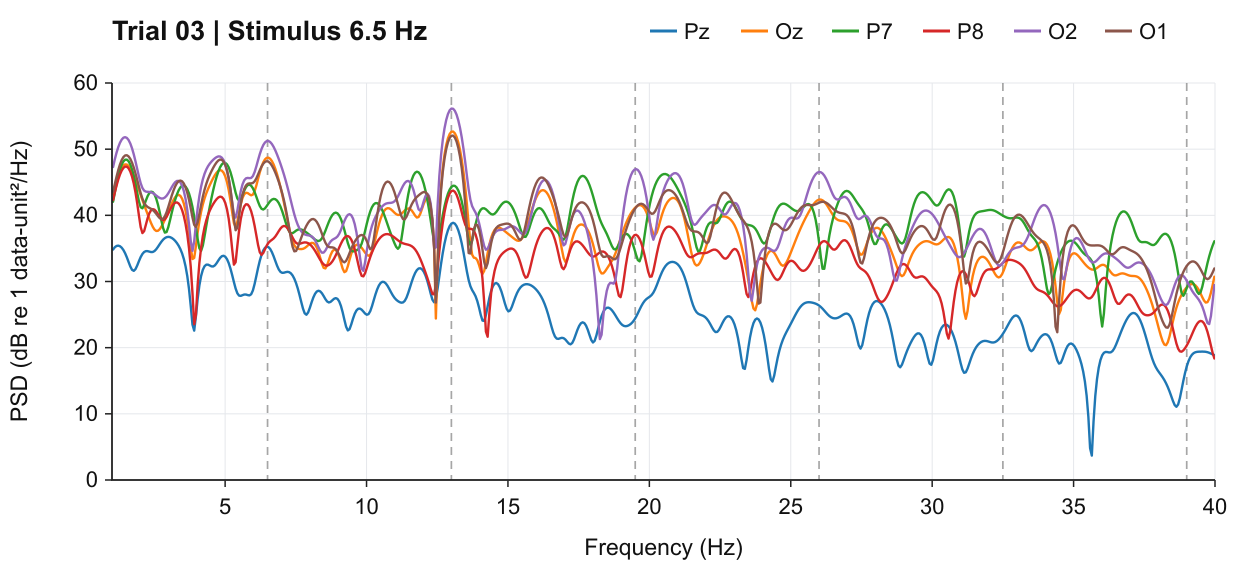
\includegraphics[width=0.9\textwidth,height=0.4\textheight,keepaspectratio]{fig17_ssvep_trial03_6p5hz.png}
\caption{Repetition 3 with a stimulation frequency of 6.5~Hz; all six channels are shown on one axis.}
\label{fig:app17}
\end{figure}

\begin{figure}[p]
\centering
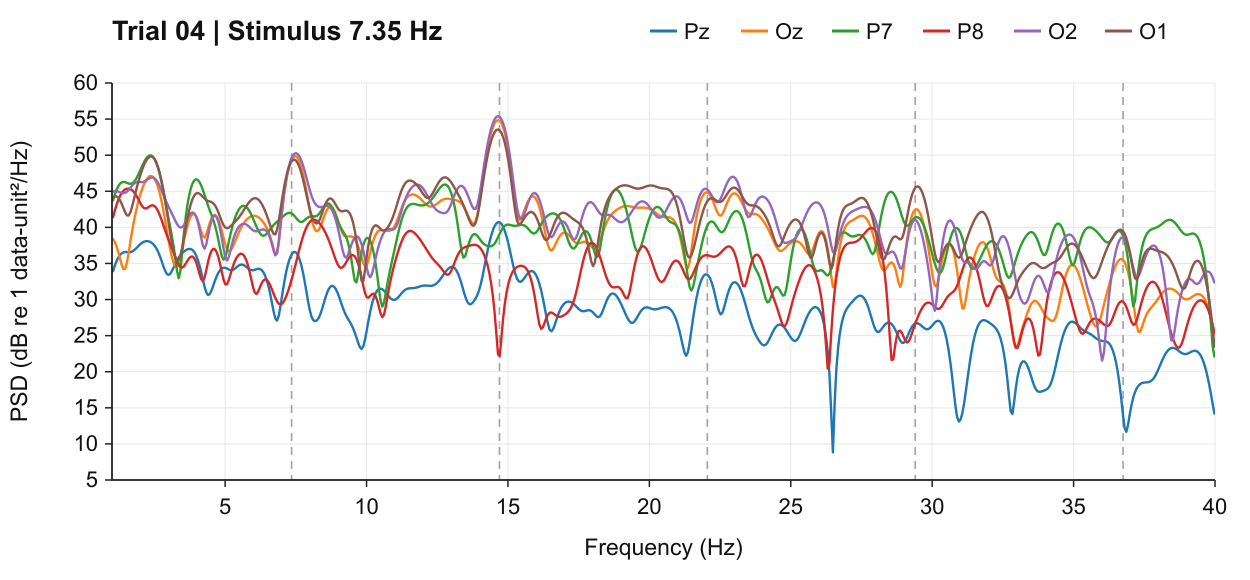
\includegraphics[width=0.9\textwidth,height=0.4\textheight,keepaspectratio]{fig18_ssvep_trial04_7p35hz.png}
\caption{Repetition 4 with a stimulation frequency of 7.35~Hz; all six channels are shown on one axis.}
\label{fig:app18}
\end{figure}

\begin{figure}[p]
\centering
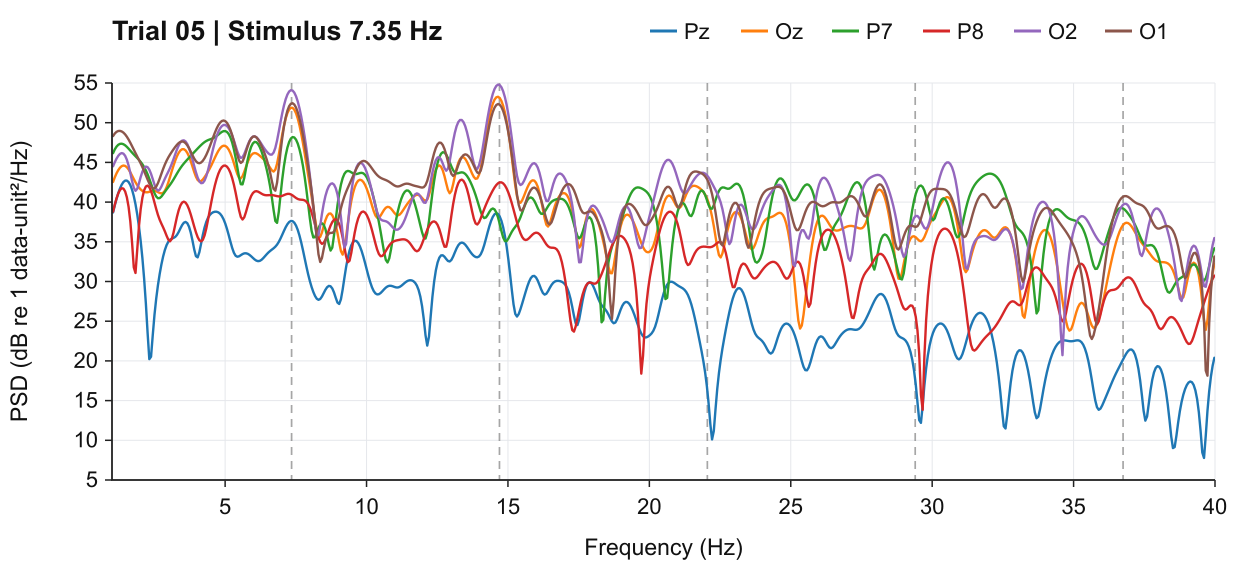
\includegraphics[width=0.9\textwidth,height=0.4\textheight,keepaspectratio]{fig19_ssvep_trial05_7p35hz.png}
\caption{Repetition 5 with a stimulation frequency of 7.35~Hz; all six channels are shown on one axis.}
\label{fig:app19}
\end{figure}

\begin{figure}[p]
\centering
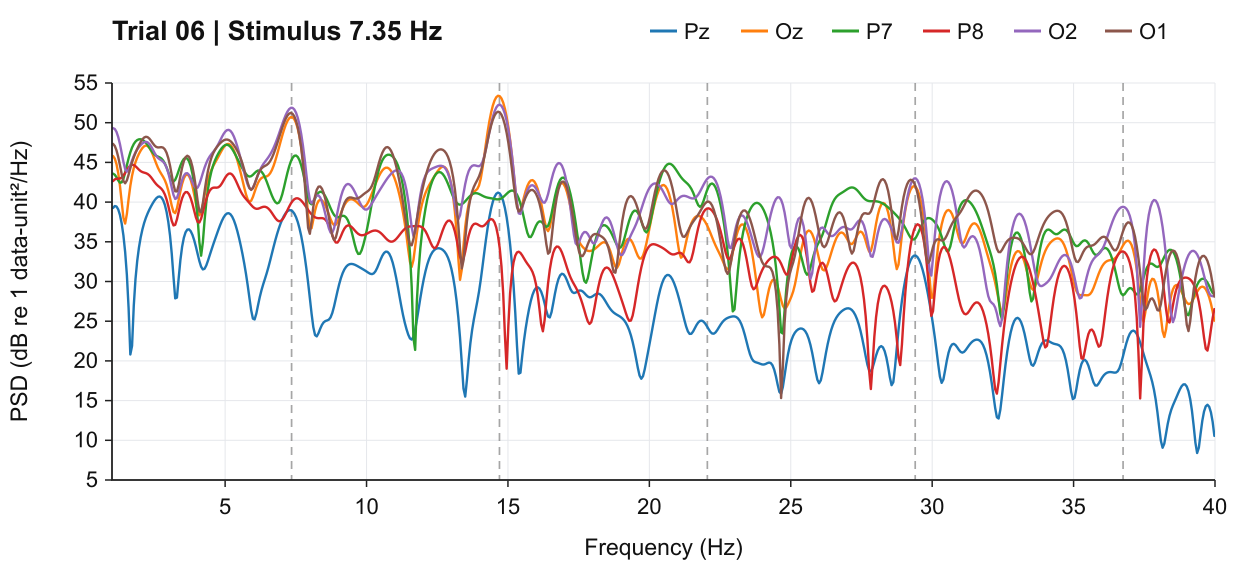
\includegraphics[width=0.9\textwidth,height=0.4\textheight,keepaspectratio]{fig20_ssvep_trial06_7p35hz.png}
\caption{Repetition 6 with a stimulation frequency of 7.35~Hz; all six channels are shown on one axis.}
\label{fig:app20}
\end{figure}

\begin{figure}[p]
\centering
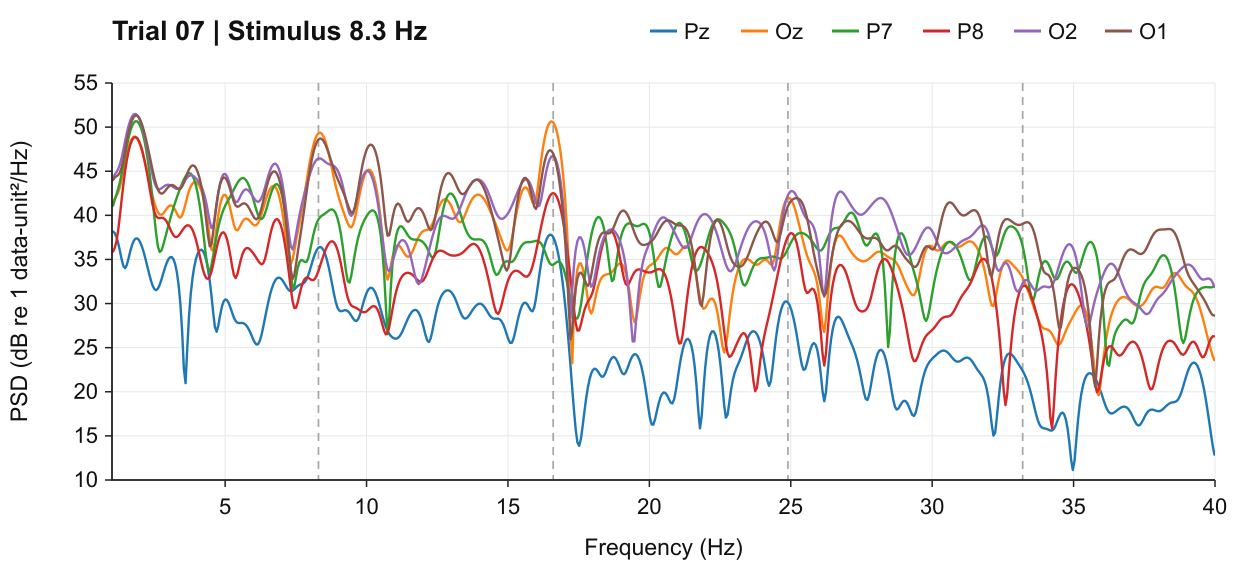
\includegraphics[width=0.9\textwidth,height=0.4\textheight,keepaspectratio]{fig21_ssvep_trial07_8p3hz.png}
\caption{Repetition 7 with a stimulation frequency of 8.3~Hz; all six channels are shown on one axis.}
\label{fig:app21}
\end{figure}

\begin{figure}[p]
\centering
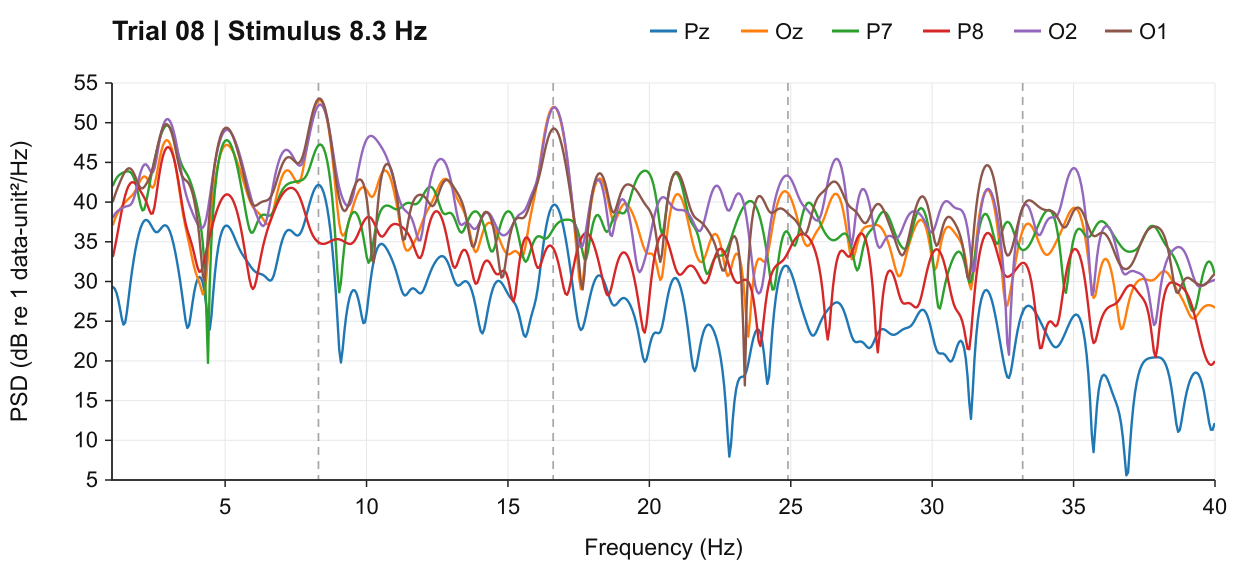
\includegraphics[width=0.9\textwidth,height=0.4\textheight,keepaspectratio]{fig22_ssvep_trial08_8p3hz.png}
\caption{Repetition 8 with a stimulation frequency of 8.3~Hz; all six channels are shown on one axis.}
\label{fig:app22}
\end{figure}

\begin{figure}[p]
\centering
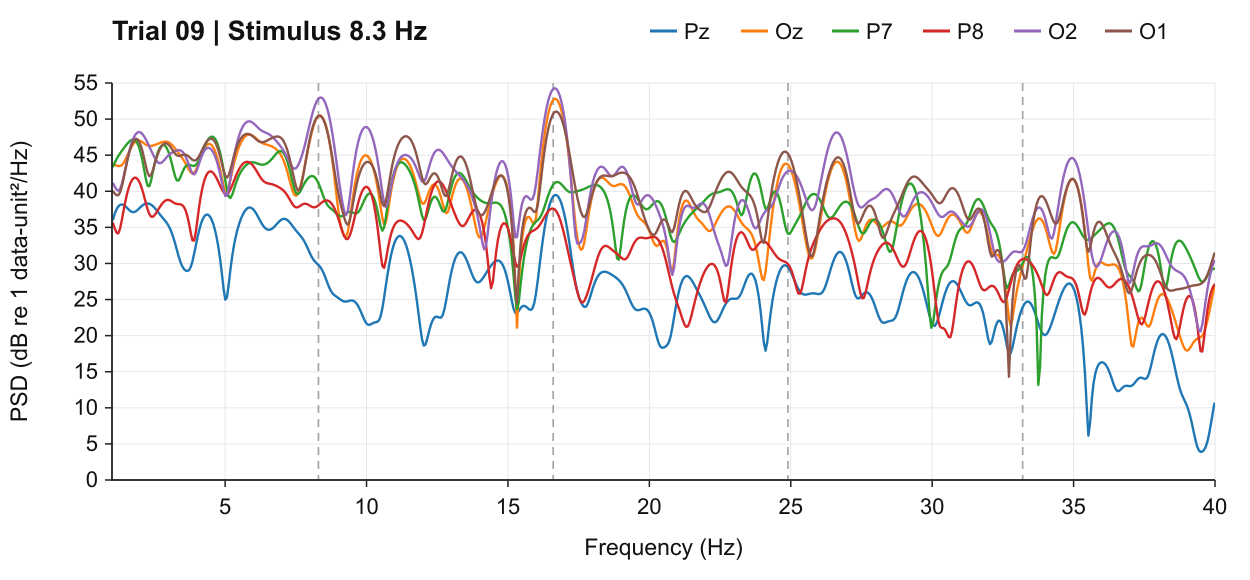
\includegraphics[width=0.9\textwidth,height=0.4\textheight,keepaspectratio]{fig23_ssvep_trial09_8p3hz.png}
\caption{Repetition 9 with a stimulation frequency of 8.3~Hz; all six channels are shown on one axis.}
\label{fig:app23}
\end{figure}

\begin{figure}[p]
\centering
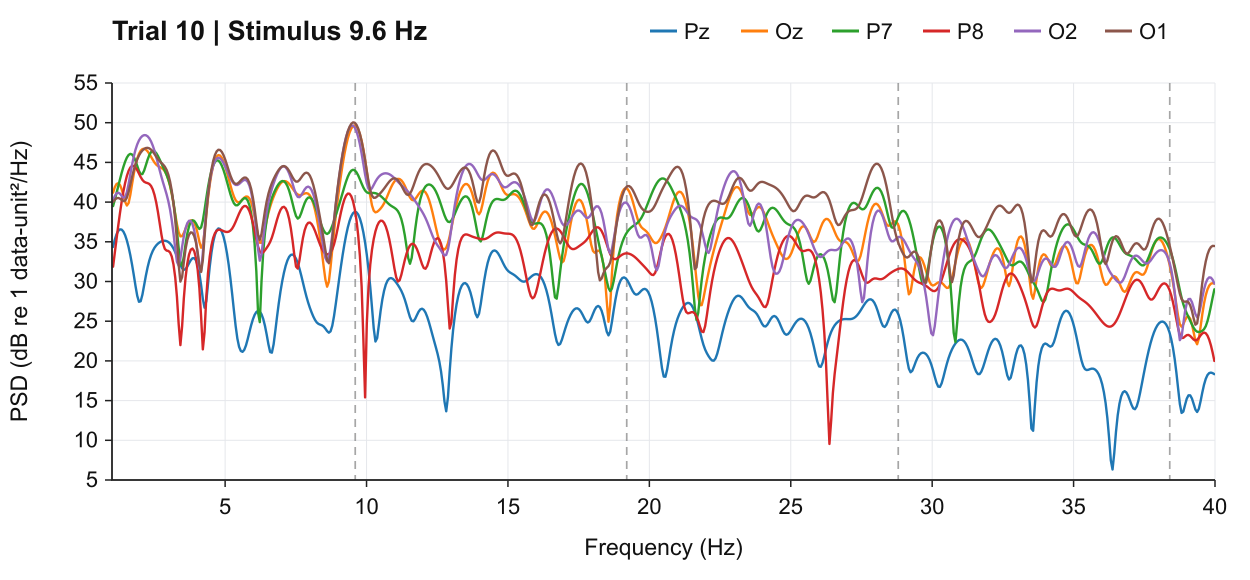
\includegraphics[width=0.9\textwidth,height=0.4\textheight,keepaspectratio]{fig24_ssvep_trial10_9p6hz.png}
\caption{Repetition 10 with a stimulation frequency of 9.6~Hz; all six channels are shown on one axis.}
\label{fig:app24}
\end{figure}

\begin{figure}[p]
\centering
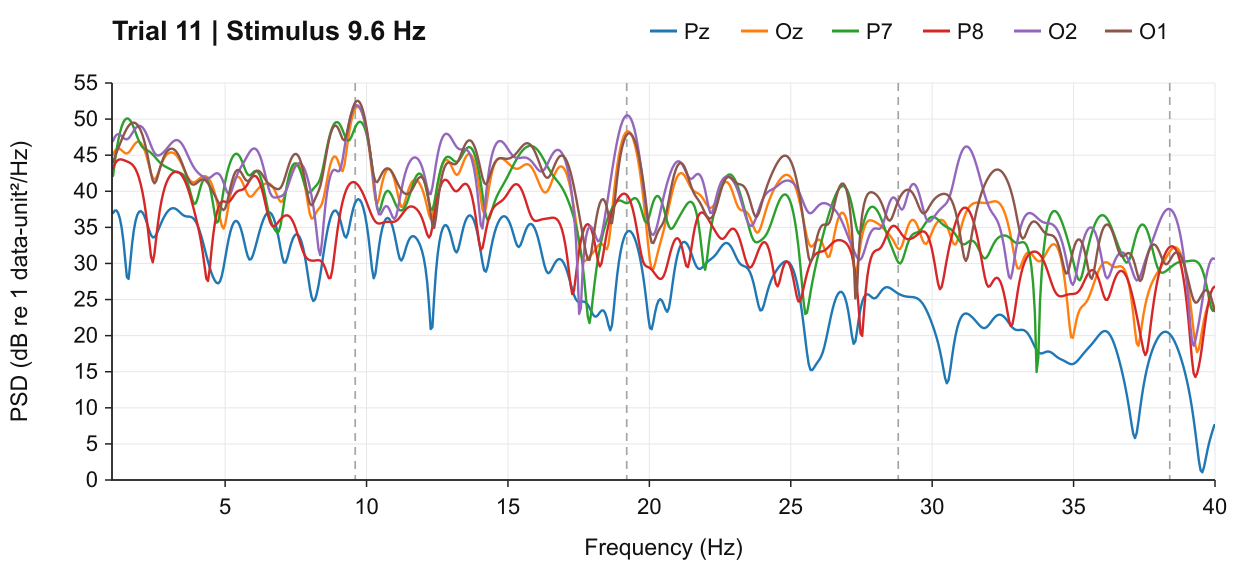
\includegraphics[width=0.9\textwidth,height=0.4\textheight,keepaspectratio]{fig25_ssvep_trial11_9p6hz.png}
\caption{Repetition 11 with a stimulation frequency of 9.6~Hz; all six channels are shown on one axis.}
\label{fig:app25}
\end{figure}

\begin{figure}[p]
\centering
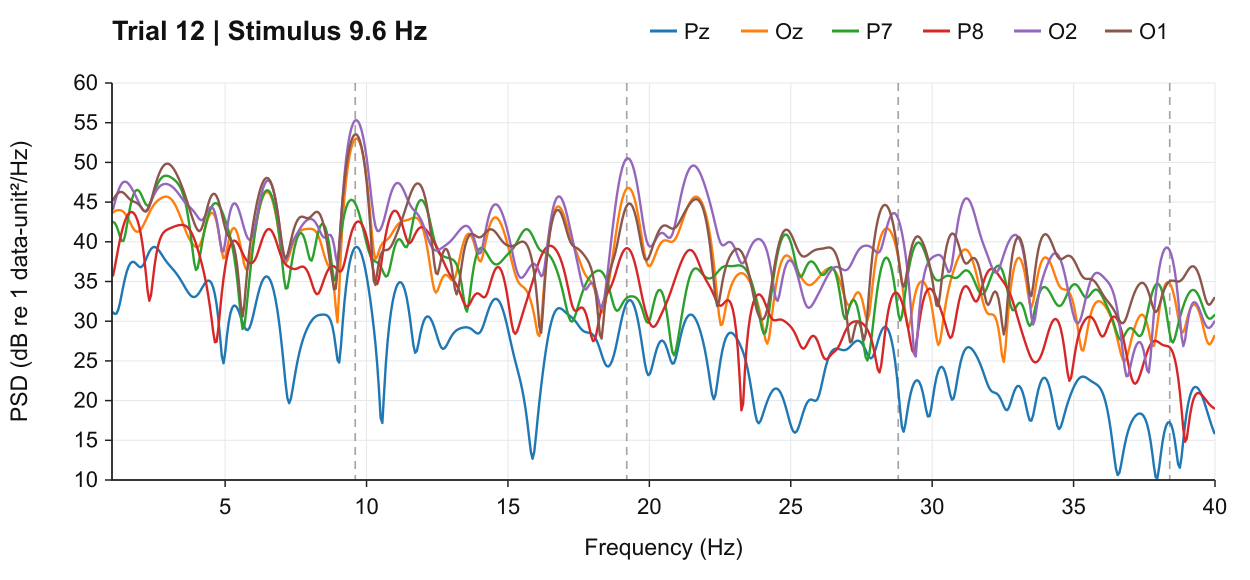
\includegraphics[width=0.9\textwidth,height=0.4\textheight,keepaspectratio]{fig26_ssvep_trial12_9p6hz.png}
\caption{Repetition 12 with a stimulation frequency of 9.6~Hz; all six channels are shown on one axis.}
\label{fig:app26}
\end{figure}

\begin{figure}[p]
\centering
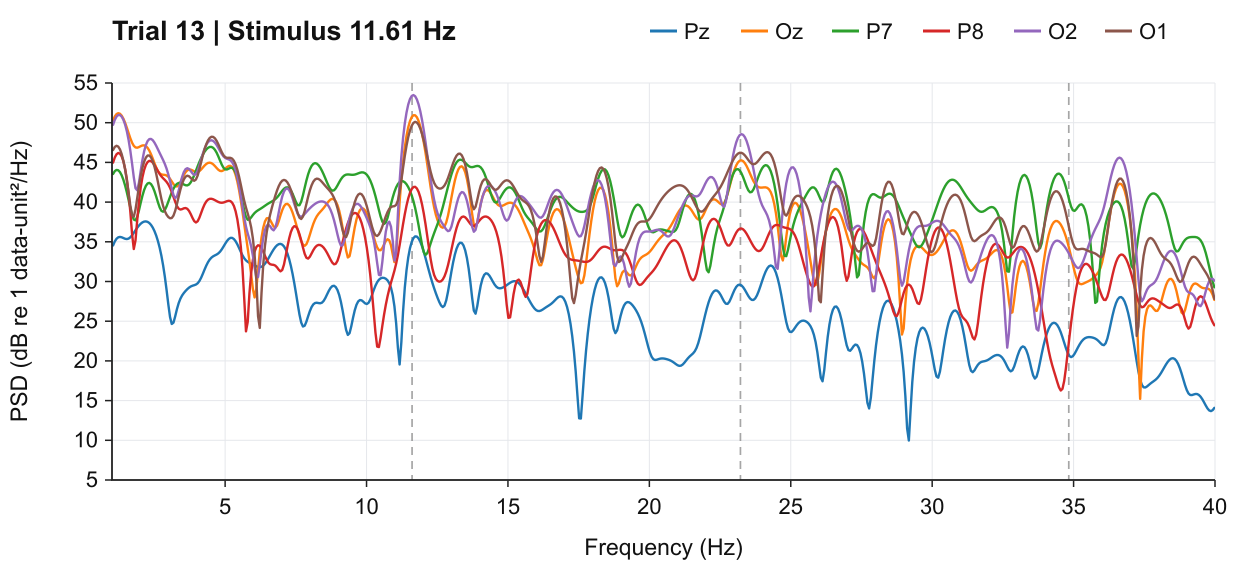
\includegraphics[width=0.9\textwidth,height=0.4\textheight,keepaspectratio]{fig27_ssvep_trial13_11p61hz.png}
\caption{Repetition 13 with a stimulation frequency of 11.61~Hz; all six channels are shown on one axis.}
\label{fig:app27}
\end{figure}

\begin{figure}[p]
\centering
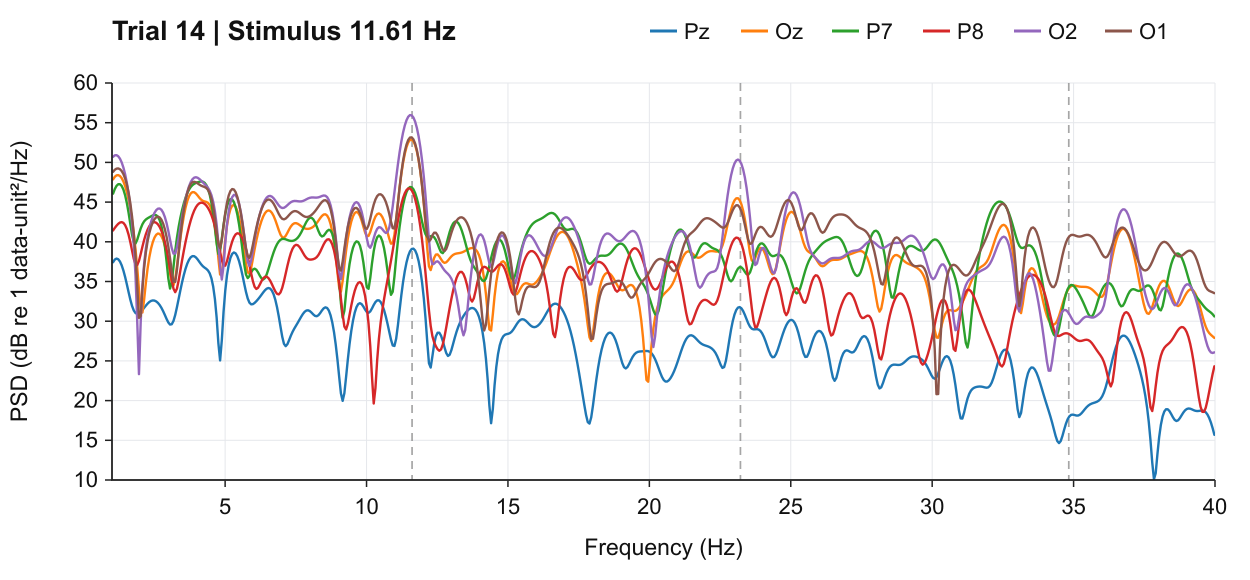
\includegraphics[width=0.9\textwidth,height=0.4\textheight,keepaspectratio]{fig28_ssvep_trial14_11p61hz.png}
\caption{Repetition 14 with a stimulation frequency of 11.61~Hz; all six channels are shown on one axis.}
\label{fig:app28}
\end{figure}

\begin{figure}[p]
\centering
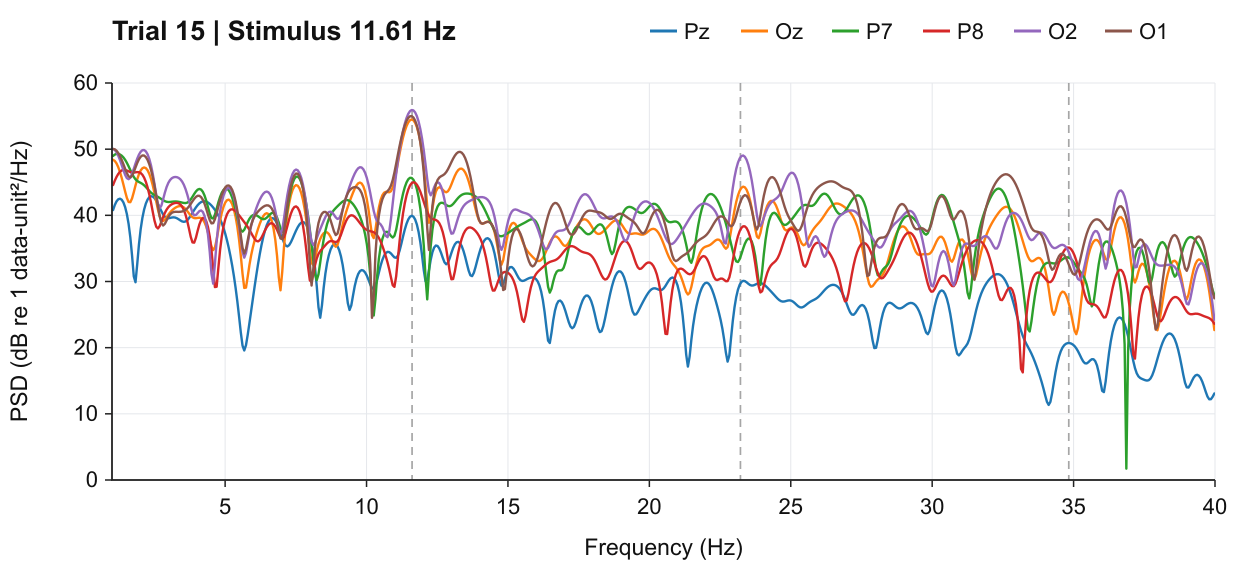
\includegraphics[width=0.9\textwidth,height=0.4\textheight,keepaspectratio]{fig29_ssvep_trial15_11p61hz.png}
\caption{Repetition 15 with a stimulation frequency of 11.61~Hz; all six channels are shown on one axis.}
\label{fig:app29}
\end{figure}

\begin{figure}[p]
\centering
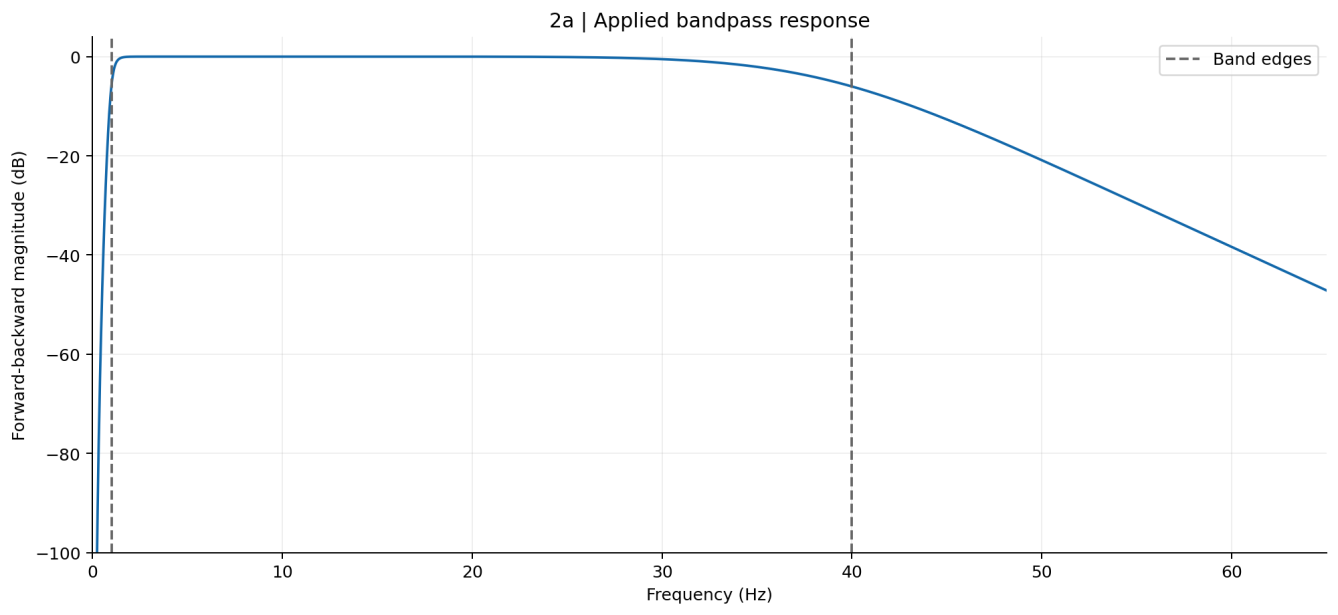
\includegraphics[width=0.9\textwidth,height=0.4\textheight,keepaspectratio]{fig30_zero_phase_filter_response.png}
\caption{Amplitude response of the forward--backward filter applied in Part~2; the transition on the two sides of the band is gradual.}
\label{fig:app30}
\end{figure}

\end{document}
